\newpage
\chapter{Analisis dan Perancangan} \label{Bab III}

\section{Alur Penelitian} \label{III.Alur}
Alur penelitian menggambarkan tahapan yang diikuti dalam proses pelaksanaan penelitian identifikasi penyakit pada bibit daun kelapa sawit dengan menggunakan ekstraksi fitur warna dan bentuk dengan metode \textit{Naïve Bayes} untuk proses identifikasinya, optimasi menggunakan \textit{Genetic Algorithm} dan \textit{Particle Swarm Optimization}.

Berikut adalah gambaran visual dari alur penelitian yang akan dilakukan dalam studi ini, seperti yang terlihat pada Gambar \ref{fig:2.Diagram Alur Penelitian}. \par
\begin{figure}[H]
	\centering
	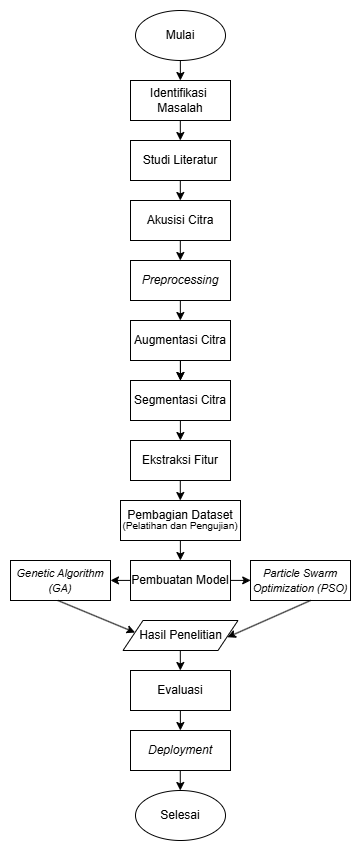
\includegraphics[width=0.3\textwidth]{figure/chapter-3-alur-penelitian.png}
	\caption{Diagram Alur Penelitian}
	\label{fig:2.Diagram Alur Penelitian}
\end{figure}

\section{Penjabaran Langkah Penelitian} \label{III.Jabar Alur}
Penjabaran langkah-langkah penelitian yang dilakukan dalam penelitian ini. Penjelasan langkah-langkah penelitian ini akan menjelaskan secara rinci setiap langkah yang diambil dalam penelitian ini, sudah tergambar dalam flowchart di subbab \ref{III.Alur}.\par


\subsection{Identifikasi Masalah} \label{III.Identifikasi Masalah}
Tahap identifikasi masalah dalam penelitian ini diawali dengan pelaksanaan observasi lapangan secara sistematis dan wawancara mendalam di PT Perkebunan Nusantara IV Regional 7 Kebun Bekri, Lampung Tengah. Observasi dilakukan pada area pembibitan kelapa sawit (\textit{Elaeis guineensis Jacq}) dengan rentang umur bibit 1 minggu hingga 3 bulan, guna mengidentifikasi secara langsung berbagai gejala patologis yang muncul pada daun bibit. Proses observasi difokuskan pada deteksi dini penyakit yang menyerang daun bibit, termasuk perubahan morfologi, perubahan warna, serta pola penyebaran gejala pada populasi bibit.

Selain observasi, dilakukan pula wawancara dengan tenaga ahli agronomi dan petugas lapangan yang memiliki pengalaman langsung dalam pengelolaan pembibitan kelapa sawit. Wawancara ini bertujuan untuk memperoleh data primer terkait karakteristik gejala penyakit, faktor-faktor penyebab, serta pola penyebaran penyakit pada bibit kelapa sawit. Informasi yang diperoleh dari wawancara digunakan untuk memperkuat temuan observasi lapangan dan memastikan validitas data yang dikumpulkan.

Hasil identifikasi menunjukkan bahwa terdapat lima kategori utama penyakit yang sering menyerang daun bibit kelapa sawit di lokasi penelitian, yaitu: bercak daun, daun menguning, daun menggulung, daun berputar, dan daun berkerut. Setiap kategori penyakit memiliki karakteristik gejala yang berbeda, baik dari segi bentuk, warna, maupun pola penyebarannya. 

\subsection{Studi Literatur} \label{III.Studi Literatur}
Studi literatur dalam penelitian ini dilakukan secara sistematis melalui penelusuran sumber-sumber akademis terpilih, seperti jurnal ilmiah, buku referensi, artikel prosiding konferensi, dan publikasi terbaru yang relevan dengan topik penelitian. Referensi yang dikaji difokuskan pada tiga aspek utama, yaitu (1) metode identifikasi penyakit tanaman berbasis citra digital, khususnya pada bibit kelapa sawit, (2) teknik ekstraksi fitur warna dan bentuk pada citra daun, dan (3) penerapan dan optimasi algoritma \textit{Naïve Bayes, Genetic Algorithm}, dan \textit{Particle Swarm Optimization} dalam klasifikasi dan pengenalan pola penyakit tanaman.

Proses studi literatur diawali dengan penentuan kata kunci yang relevan, seperti "identifikasi penyakit bibit daun kelapa sawit", "ekstraksi fitur warna dan bentuk", "Naïve Bayes", "Genetic Algorithm", dan "Particle Swarm Optimization". Selanjutnya, dilakukan pencarian literatur pada basis data ilmiah seperti IEEE Xplore, ScienceDirect, SpringerLink, dan Google Scholar. Setiap literatur yang diperoleh dianalisis untuk mengidentifikasi perkembangan metode, kelebihan dan keterbatasan pendekatan yang telah ada, serta peluang inovasi yang dapat diadopsi dalam penelitian ini.

Hasil studi literatur menjadi dasar dalam merumuskan metodologi penelitian dan tinjauan pustaka, menentukan parameter dan teknik yang digunakan, serta membandingkan hasil penelitian dengan studi terdahulu untuk menilai kontribusi dan keunggulan pendekatan yang diusulkan.

\subsection{Akuisisi Dataset Citra} \label{III.Akuisisi Citra}
Pengumpulan dataset dilakukan secara langsung di area pembibitan PT Perkebunan Nusantara IV Regional 7 Kebun Bekri, Lampung Tengah, sesuai prosedur perizinan dari pihak perusahaan. Data citra daun bibit kelapa sawit diambil dengan mengelompokkan sesuai lima kategori penyakit utama yang telah diidentifikasi, serta daun sehat sebagai pembanding.

Pengambilan citra dilakukan menggunakan kamera Canon EOS700D pada jarak sekitar 20 cm dari objek daun. Untuk menjaga konsistensi dan memudahkan proses segmentasi, digunakan kertas HVS putih sebagai latar belakang saat pengambilan gambar. Setiap citra diambil dengan memperhatikan variasi sudut dan pencahayaan agar dataset yang dihasilkan representatif.

Seluruh citra yang diperoleh diberi label sesuai kategori penyakit berdasarkan hasil observasi dan konfirmasi tenaga ahli agronomi. Dataset citra disimpan dalam format JPEG/PNG dan diorganisasi ke dalam folder sesuai kelas penyakit untuk memudahkan proses ekstraksi fitur dan pelatihan model klasifikasi. Ilustrasi teknik pengambilan dataset citra daun bibit kelapa sawit dapat dilihat pada Gambar \ref{fig:3.Ilustrasi Akuisisi}.

\begin{figure}[H]
	\centering
	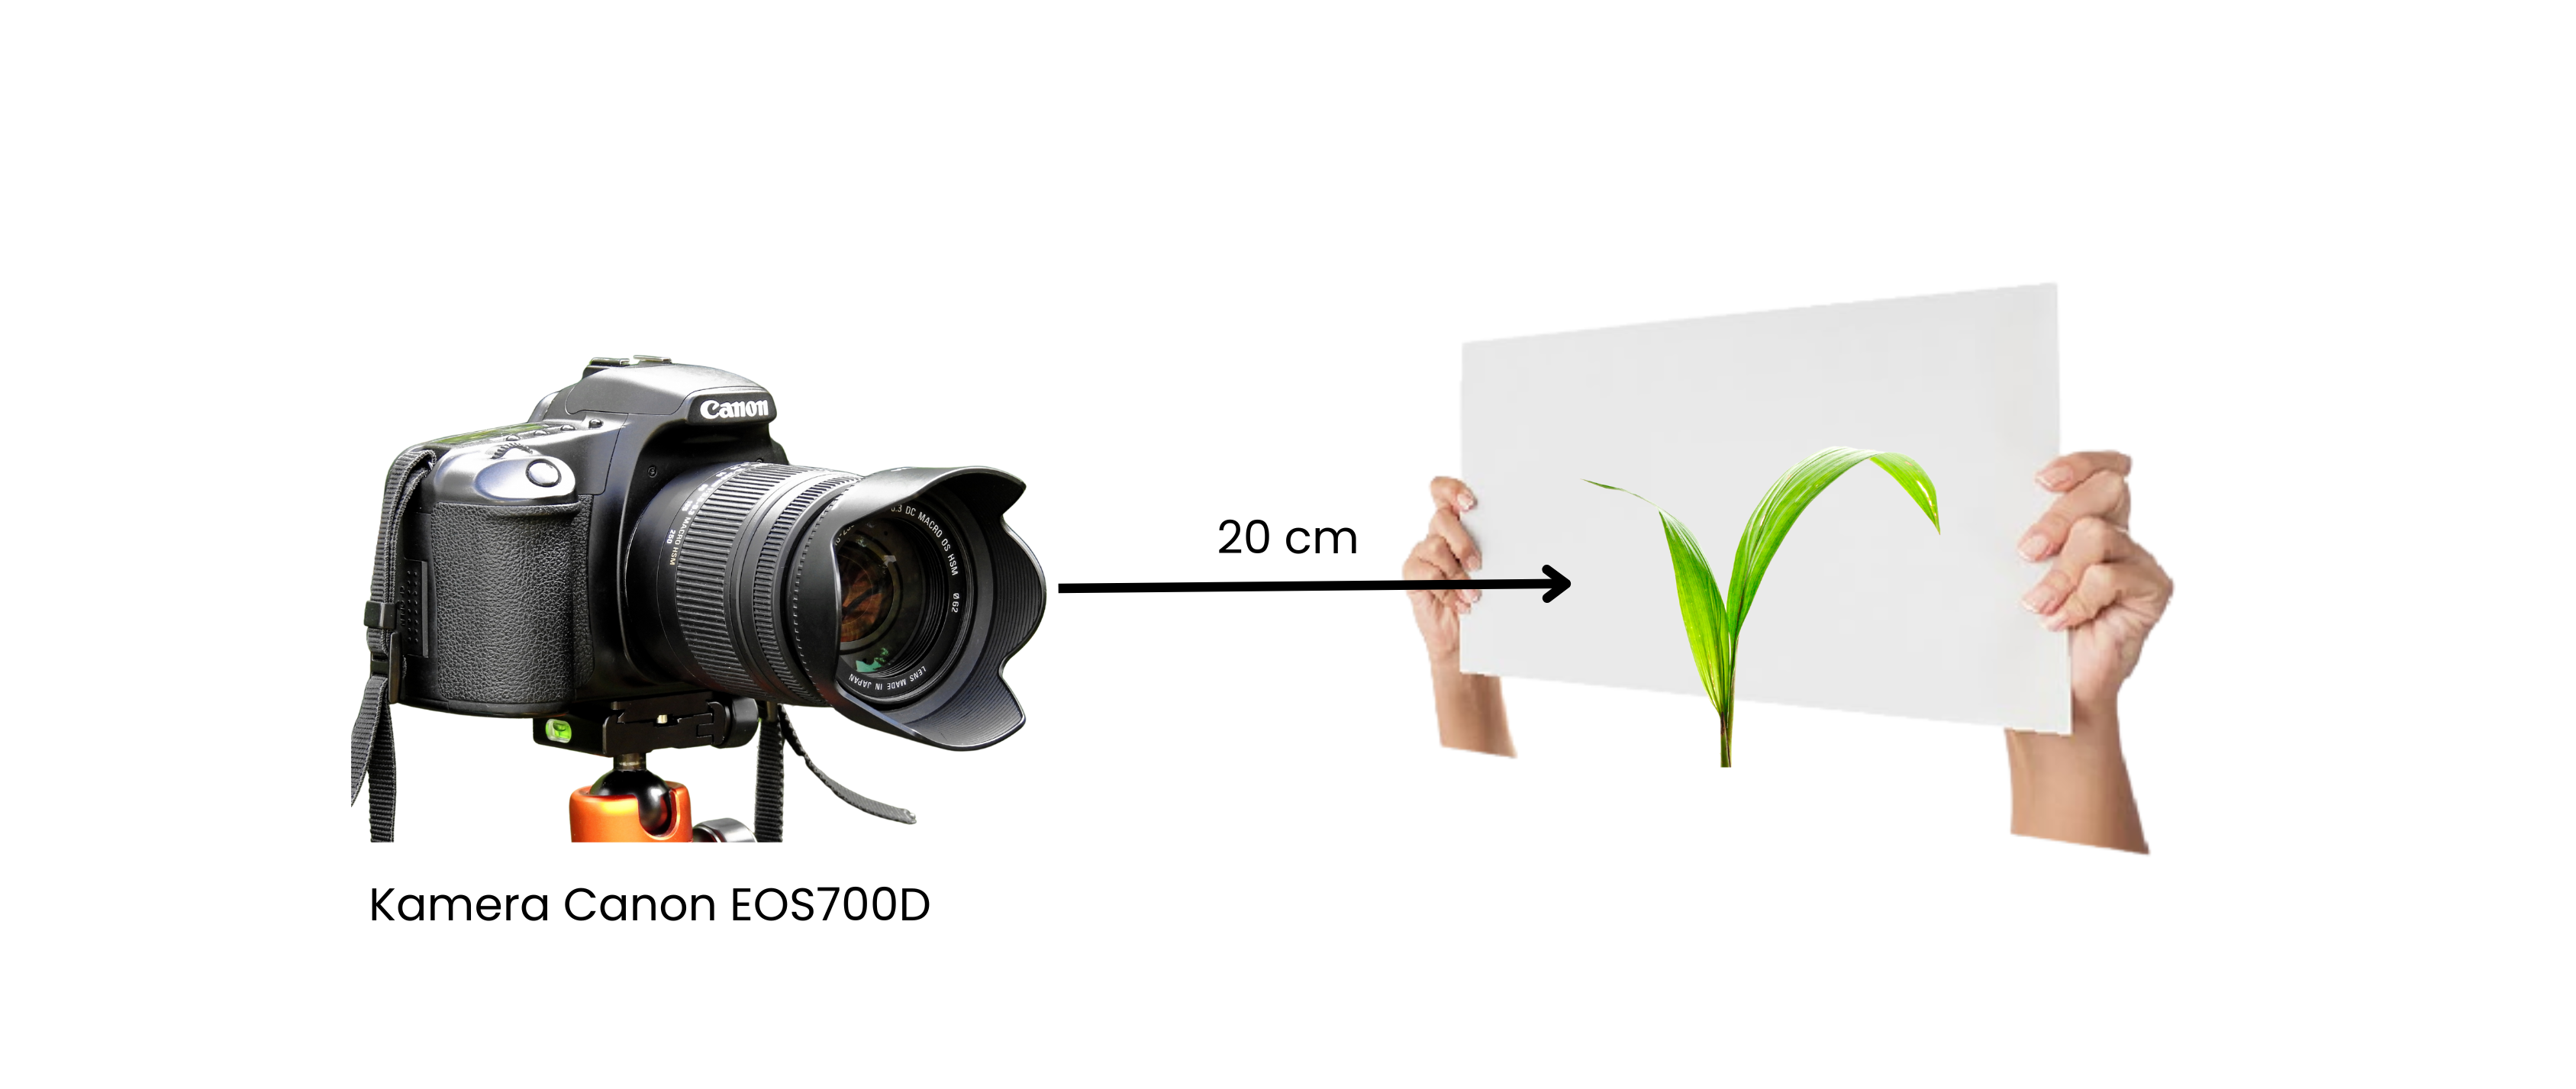
\includegraphics[width=1\textwidth]{figure/chapter-3-ilustrasi-akuisisi.png}
	\caption{Ilustrasi Pengambilan Dataset Daun Bibit Kelapa Sawit}
	\label{fig:3.Ilustrasi Akuisisi}
\end{figure}

\subsection{\textit{Preprocessing}} \label{III.Preprocessing }
Dataset yang telah diakuisisi selanjutnya melalui tahap \textit{preprocessing} untuk memastikan kualitas data sebelum digunakan dalam pelatihan model. \textit{Preprocessing} bertujuan meningkatkan konsistensi dan akurasi data citra, sehingga fitur yang diekstraksi menjadi lebih representatif.

Tahapan \textit{preprocessing} yang dilakukan meliputi penghapusan latar belakang untuk memudahkan deteksi objek utama, yaitu daun kelapa sawit. Selanjutnya, dilakukan \textit{cropping} untuk memfokuskan area citra pada objek daun, diikuti dengan proses resizing agar seluruh citra memiliki dimensi seragam. Pada penelitian ini, citra diubah ke ukuran 256 x 256 piksel dengan rasio 1:1, menyesuaikan kebutuhan model \textit{Naive Bayes}. Setelah itu, normalisasi dilakukan menggunakan nilai rata-rata (mean) dan standar deviasi \textit{(standard deviation)} agar distribusi intensitas piksel seragam dan tidak terpengaruh variasi pencahayaan.

Dengan tahapan \textit{preprocessing} ini, diharapkan data citra yang digunakan pada proses ekstraksi fitur dan pelatihan model menjadi lebih optimal dan siap untuk tahap analisis selanjutnya.

\subsection{Augmentasi Citra} \label{III.Augmentasi Citra}
Augmentasi citra dilakukan untuk memperbanyak jumlah data pelatihan dan meningkatkan keragaman dataset. Proses ini bertujuan untuk mengurangi risiko \textit{overfitting} pada model klasifikasi yang dibangun. Probabilitas augmentasi citra ini disusun secara paralel pada platform Roboflow, yang menyediakan berbagai teknik augmentasi citra secara otomatis.

Dalam platform Roboflow, transformasi augmentasi diterapkan menggunakan pendekatan probabilistik (misalnya p=0.5 untuk rotasi), menghasilkan variasi data lebih komprehensif dibandingkan metode deterministik konvensional. Sebagai contoh, jika rotasi 90° diterapkan dengan probabilitas 0.5 (50\%), maka hanya sekitar setengah dari gambar dataset akan mengalami transformasi rotasi tersebut. 

Pendekatan stokastik ini kritis untuk mencegah bias sistematis dan membangun model robust. Pada identifikasi patologi daun kelapa sawit, augmentasi probabilistik memungkinkan model mengakomodasi variabilitas morfologis penyakit, termasuk variasi sudut, orientasi, dan pencahayaan yang menyerupai kondisi lapangan. Konfigurasi multi-probabilitas menciptakan ruang fitur yang lebih kaya, meningkatkan kapasitas generalisasi terhadap kondisi tidak terkontrol. Transformasi independen pada setiap citra memperkaya distribusi data pelatihan tanpa menambah beban akuisisi data primer.

Penyusunan probabilitas paralel ini memungkinkan setiap citra dalam dataset mengalami beberapa transformasi secara acak, sehingga menghasilkan variasi citra yang berbeda dari citra asli. Dengan demikian, model dapat belajar mengenali pola penyakit dari berbagai sudut pandang dan kondisi pencahayaan yang berbeda.

Augmentasi dilakukan dengan menerapkan beberapa teknik, antara lain rotasi, \textit{flipping, shear}, dan perubahan kecerahan. Teknik rotasi dilakukan dengan memutar citra pada sudut tertentu, teknik \textit{flipping} dilakukan dengan membalik citra secara horizontal atau vertikal, teknik shear adalah teknik yang mengubah perspektif citra dengan menggeser piksel pada sumbu x atau y, sehingga menghasilkan efek miring, sedangkan perubahan kecerahan dilakukan dengan menyesuaikan nilai intensitas piksel pada citra.

\subsubsection{Rotasi} \label{III.Rotasi}
Rotasi citra dilakukan dengan memutar citra pada sudut tertentu, misalnya 90, 180, atau 270 derajat. Proses ini bertujuan untuk menghasilkan variasi citra yang berbeda dari citra asli, sehingga model dapat belajar mengenali pola penyakit dari berbagai sudut pandang.
\begin{figure}[H]
	\centering
	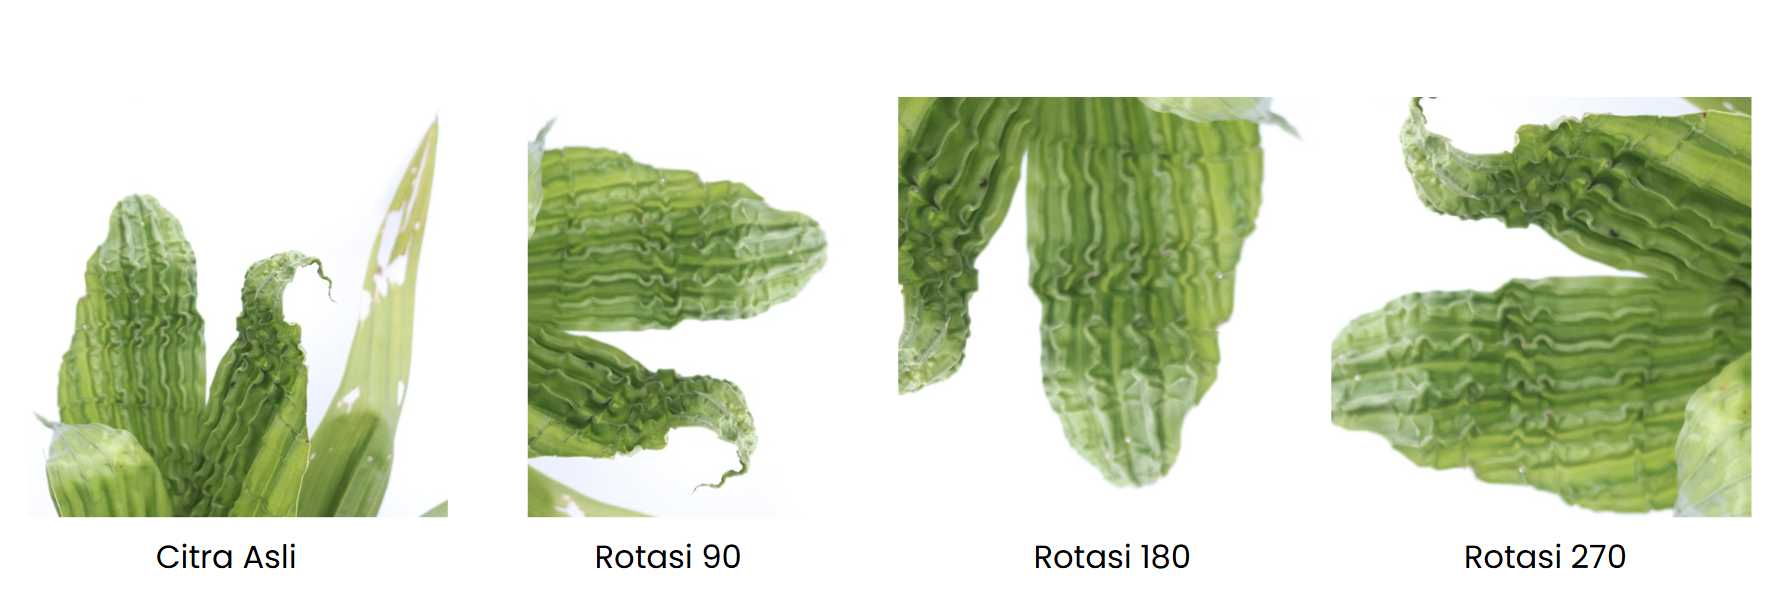
\includegraphics[width=0.5\textwidth]{figure/chapter-3-rotasi.png}
	\caption{Ilustrasi Rotasi Citra}
	\label{fig:3.Rotasi}
\end{figure}

\subsubsection{Flipping} \label{III.Flipping}
\textit{Flipping} citra dilakukan dengan membalik citra secara horizontal atau vertikal. Teknik ini bertujuan untuk menghasilkan variasi citra yang berbeda dari citra asli, sehingga model dapat belajar mengenali pola penyakit dari berbagai sudut pandang.
\begin{figure}[H]
	\centering
	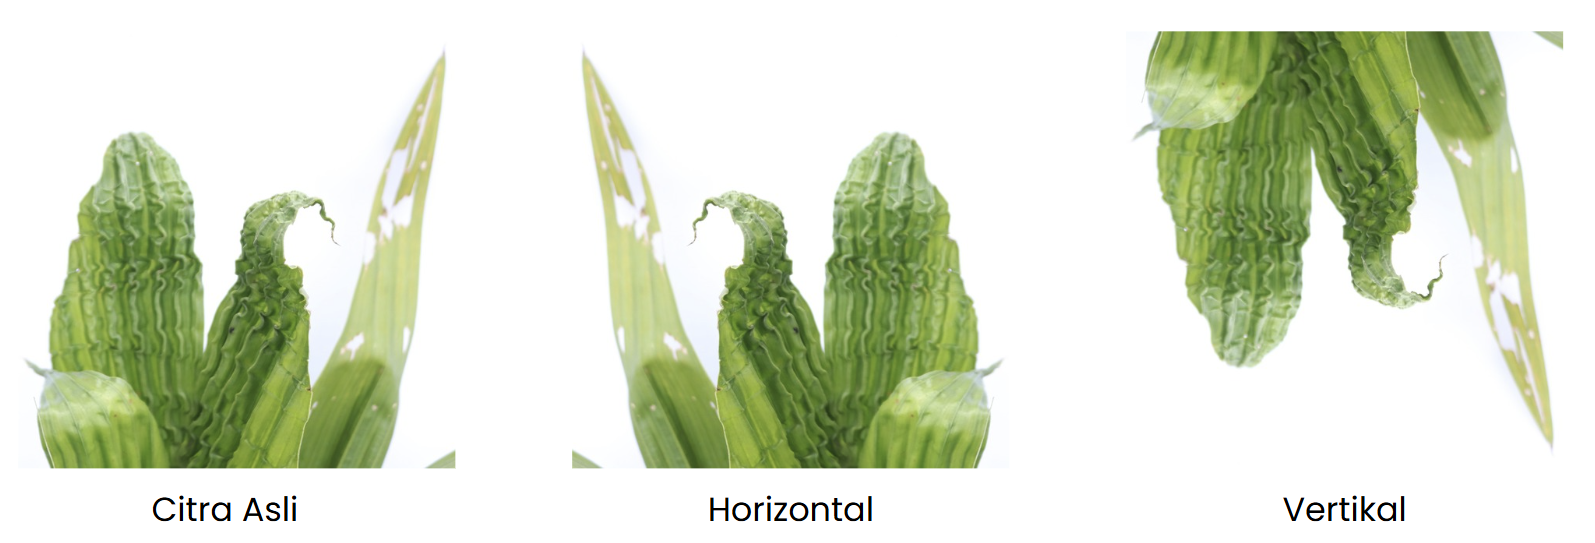
\includegraphics[width=0.5\textwidth]{figure/chapter-3-flipping.png}
	\caption{Ilustrasi Flipping Citra}
	\label{fig:3.Flipping}
\end{figure}

\subsubsection{Shear} \label{III.Shear}
\textit{Shear} adalah teknik yang mengubah perspektif citra dengan menggeser piksel pada sumbu x atau y, sehingga menghasilkan efek miring. Teknik ini bertujuan untuk menghasilkan variasi citra yang berbeda dari citra asli, sehingga model dapat belajar mengenali pola penyakit dari berbagai sudut pandang.

\subsubsection{Perubahan Kecerahan} \label{III.Kecerahan}
Perubahan kecerahan dilakukan dengan menyesuaikan nilai intensitas piksel pada citra. Teknik ini bertujuan untuk menghasilkan variasi citra yang berbeda dari citra asli, sehingga model dapat belajar mengenali pola penyakit dari berbagai sudut pandang.
\begin{figure}[H]
	\centering
	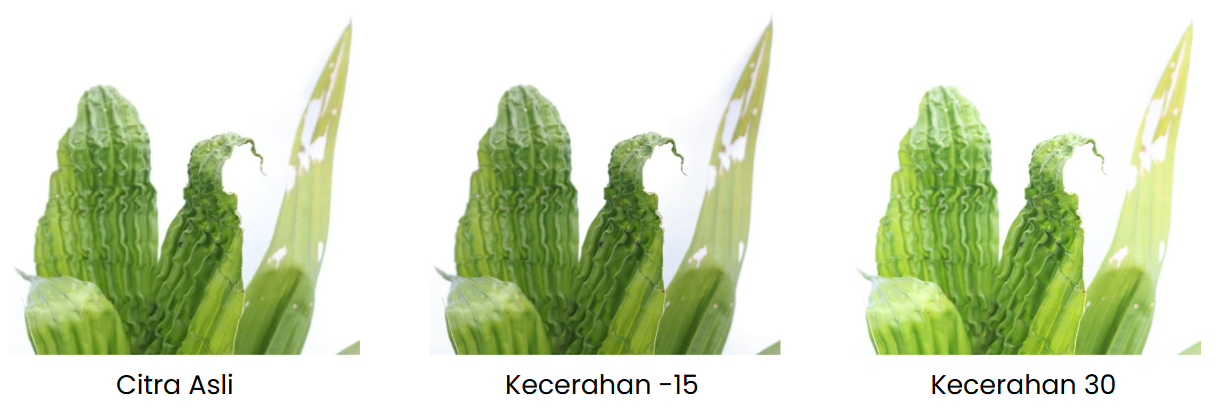
\includegraphics[width=0.5\textwidth]{figure/chapter-3-kecerahan.png}
	\caption{Ilustrasi Perubahan Kecerahan Citra}
	\label{fig:3.Kecerahan}
\end{figure}

\subsection{Segmentasi Citra} \label{III.Segmentasi Citra}
Segmentasi Citra merupakan proses pemisahan objek dari latar belakang dalam citra. Pada penelitian ini, segmentasi dilakukan untuk memisahkan bibit daun kelapa sawit dari latar belakang putih yang digunakan saat pengambilan gambar. Proses segmentasi yang dilakukan pada penelitian ini adalah dengan cara manual dengan memakai Website Photoroom yang dapat menghapus latar belakang pada citra daun kelapa sawit. Dengan menggunakan metode ini, diharapkan hasil segmentasi dapat lebih akurat dan memudahkan proses ekstraksi fitur selanjutnya.
\begin{figure}[H]
	\centering
	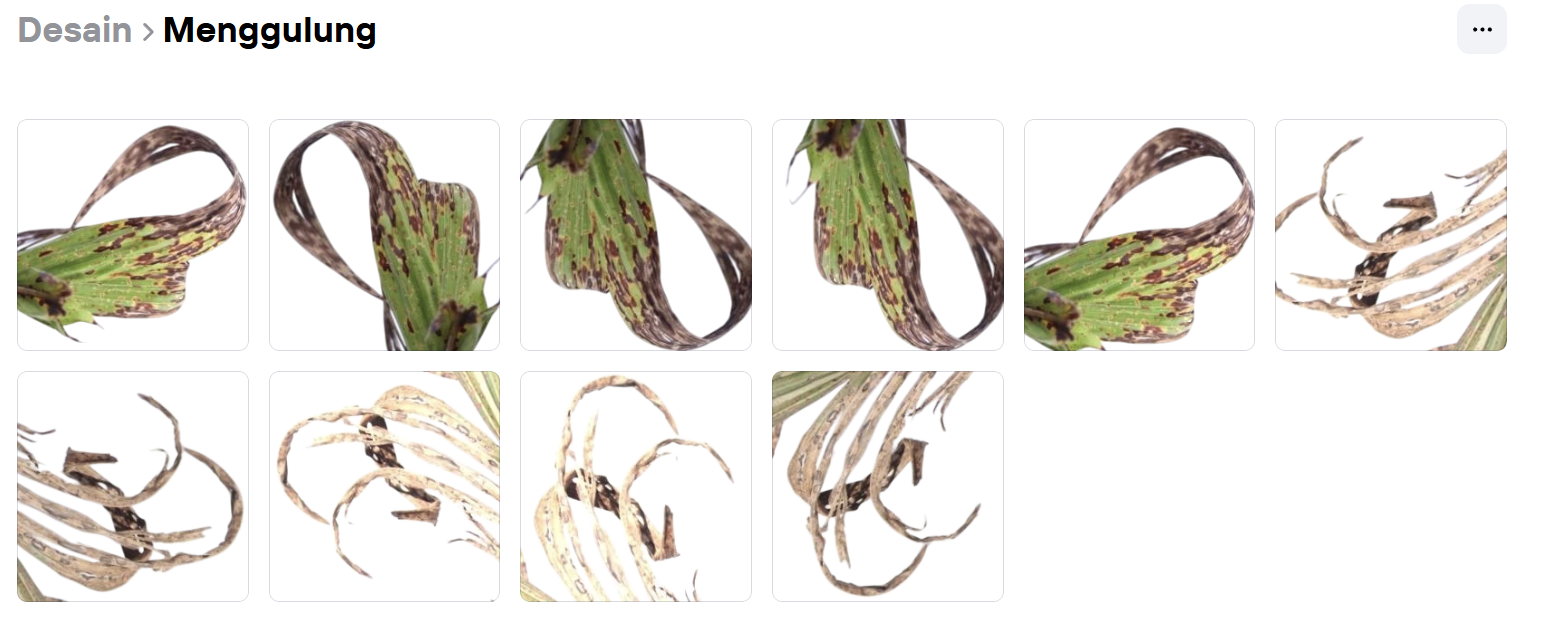
\includegraphics[width=0.5\textwidth]{figure/chapter-3-segmentasi-citra.png}
	\caption{Ilustrasi Segmentasi Citra}
	\label{fig:3.Segmentasi Citra}
\end{figure}

\subsection{Ekstraksi Fitur} \label{III.Ekstraksi Fitur}
Ekstraksi fitur merupakan langkah dalam proses pengenalan pola, di mana fitur-fitur yang relevan diambil dari citra daun untuk digunakan dalam pembuatan model. Pada penelitian ini, dua jenis fitur diekstraksi, yaitu fitur warna dan fitur bentuk.

Ekstraksi fitur warna menggunakan klasifikasi hex code RGB dan ekstraksi fitur tekstur menggunakan metode GLCM. Pada ekstraksi warna, dilakukan perhitungan rata-rata nilai RGB dari setiap citra dan keseluruhan dataset, sementara untuk tekstur, citra dikonversi ke \textit{grayscale} untuk menganalisis karakteristik seperti kontras, korelasi, energi, dan homogenitas menggunakan GLCM. Hasil ekstraksi fitur ini kemudian digunakan dalam proses klasifikasi menggunakan metode \textit{Naïve Bayes}, di mana dilakukan perhitungan nilai rata-rata, standar deviasi, \textit{prior probability}, dan \textit{posterior probability} untuk setiap kelas.

Fitur-fitur yang diekstraksi kemudian digabungkan menjadi vektor fitur tunggal untuk setiap citra. Vektor fitur ini akan digunakan sebagai input pada model yang dibangun.

\subsection{Pembagian Dataset} \label{III.Pembagian Dataset}
Pembagian Dataset dilakukan untuk memisahkan data menjadi dua bagian, yaitu data pelatihan dan data pengujian. Data pelatihan digunakan untuk melatih model klasifikasi, sedangkan data pengujian digunakan untuk mengukur kinerja model setelah dilatih.

Pada penelitian ini, pembagian dataset dilakukan dengan proporsi 80:20, di mana 80\% dari total dataset digunakan sebagai data pelatihan dan 20\% sebagai data pengujian. Pembagian ini bertujuan untuk memastikan bahwa model yang dibangun dapat generalisasi dengan baik terhadap data baru yang belum pernah dilihat sebelumnya.

\subsection{Pembuatan Model} \label{III.Pembuatan Model}
Pembuatan model dilakukan dengan menggunakan metode algoritma \textit{Naïve Bayes}, optimasi \textit{Genetic Algorithm} dan \textit{Particle Swarm Optimization}. Model \textit{Naïve Bayes} digunakan untuk identifikasi penyakit berdasarkan fitur yang diekstraksi dari citra daun. Algoritma ini bekerja dengan menghitung probabilitas setiap kelas penyakit berdasarkan fitur yang ada.

\textit{Genetic Algorithm} digunakan untuk optimasi parameter model, dengan tujuan meningkatkan akurasi klasifikasi. Algoritma ini bekerja dengan cara mensimulasikan proses evolusi, di mana individu-individu dalam populasi dihasilkan melalui kombinasi dan mutasi parameter yang ada.

\textit{Particle Swarm Optimization} digunakan untuk mencari solusi optimal dalam ruang parameter model. Algoritma ini bekerja dengan cara mensimulasikan perilaku kawanan burung, di mana setiap partikel dalam kawanan bergerak menuju posisi terbaik yang ditemukan oleh individu dan kelompok.

\subsection{Hasil} \label{III.Hasil}
Hasil dari penelitian ini adalah model yang dapat mengidentifikasi penyakit pada bibit daun kelapa sawit dengan akurasi yang tinggi. Model yang dihasilkan diuji menggunakan data pengujian yang telah dipisahkan sebelumnya. 

\subsection{Evaluasi} \label{III.Evaluasi}
Tahapan evaluasi merupakan ulasan terkait penelitian yang telah dilaksanakan untuk menilai kinerja model yang telah dibuat. Evaluasi dilakukan menggunakan dua pendekatan, yaitu menggunakan \textit{confusion matrix} dan metrik evaluasi.

\textit{Confusion matrix} digunakan untuk mengukur performa model klasifikasi dengan memberikan rincian jumlah prediksi yang benar dan salah pada masing-masing kelas. Nilai-nilai yang dihasilkan dari \textit{confusion matrix} meliputi \textit{True Positive (TP), False Positive (FP), True Negative (TN)}, dan \textit{False Negative (FN)}. Berdasarkan nilai-nilai ini, dapat dihitung metrik evaluasi seperti akurasi, presisi, \textit{recall}, dan \textit{F1-score}.

Akurasi mengukur proporsi prediksi yang benar terhadap seluruh data, presisi mengukur ketepatan prediksi positif, \textit{recall} mengukur kemampuan model dalam menemukan seluruh kasus positif, dan \textit{F1-score} merupakan rata-rata harmonis dari presisi dan recall. Dengan menggunakan \textit{confusion matrix} dan metrik evaluasi tersebut, dapat diketahui seberapa baik model dalam mengidentifikasi penyakit pada bibit daun kelapa sawit. Hasil evaluasi ini menjadi dasar untuk menilai efektivitas dan keandalan model yang dihasilkan dalam penelitian.

\subsection{Deployment} \label{III.Deployment}
\textit{Deployment} adalah tahap akhir dari penelitian ini, di mana model yang telah dibangun dan diuji akan diterapkan dalam lingkungan nyata. Pada penelitian ini, deployment dilakukan dengan mengintegrasikan model ke dalam aplikasi berbasis web menggunakan Streamlit. Aplikasi web ini bertujuan untuk memudahkan pengguna dalam mengidentifikasi penyakit pada daun bibit kelapa sawit. 

Pengguna dapat mengunggah citra daun bibit kelapa sawit ke dalam aplikasi, kemudian aplikasi akan memproses citra tersebut dan memberikan hasil klasifikasi penyakit secara otomatis. Dengan adanya aplikasi ini, proses identifikasi penyakit menjadi lebih praktis dan dapat diakses oleh pengguna secara luas.

\section{Alat dan Bahan Tugas Akhir} \label{III.Alat dan Bahan}
Alat dan bahan digunakan sebagai penunjang dalam penelitian ini guna mendapatkan hasil yang optimal. Spesifikasi alat dan bahan yang digunakan dalam penelitian ini adalah sebagai berikut: \par

\subsection{Alat} \label{III.Alat}
Alat yang digunakan selama penelitian ini berlangsung, antara lain: \par
\begin{enumerate}[noitemsep]
	\item ASUS Vivobook Pro 15 OLED M3500QC-OLED956 Quiet Blue, AMD Ryzen 9 5900HX, 16GB DDR4, 512GB SSD M.2 PCIe NVMe, NVIDIA GeForce RTX 3050 4GB DDR6, 15.6" Full HD (1920x1080) OLED, Wi-Fi, Bluetooth, Webcam, Backlight Keyboard, Fingerprint, 1.65kg, Windows 11 + Office Home Student 2021.
	\item Notebook dengan spesifikasi minumum sistem operasi MacOS Sonoma 14.7, processor Apple M3, RAM 8GB, SSD 512 GB.
	\item Notebook dengan spesifikasi minimum sistem operasi Windows 11, processor AMD Ryzen 5 5560u CPU @ 6 core 12 Threads / 2.3 GHz, RAM 16GB DDR4 grafis AMD Radeon RX Vega 6 512MB, SSD 256 GB.
	\item Canon EOS 700D
	\item Kertas HVS 1 lembar
	\item Google Collab
	\item Google Drive
	\item Python 3.11.12
	\item Code editor Microsoft Visual Studio Code
	\item Github
	\item Roboflow 
	\item Streamlit
	\item Photoroom
\end{enumerate}

\subsection{Bahan} \label{III.Bahan}
Bahan yang digunakan/diperlukan untuk melakukan penelitian, dapat berupa: \par
\begin{enumerate}[noitemsep]
	\item Dataset citra daun bibit kelapa sawit yang diambil secara langsung di PT Perkebunan Nusantara IV Regional 7 Kebun Bekri, Lampung Tengah pada tanggal 6 November 2024 dan 28 Oktober 2024. Pengambilan citra menggunakan kamera Canon EOS700D dengan jarak 20 cm antara daun dan kamera, serta menggunakan kertas HVS putih sebagai latar belakang untuk memudahkan proses segmentasi. Dataset citra yang digunakan untuk model \textit{Naïve Bayes} terdiri dari 5 kelas, yaitu bercak daun sebanyak 75 citra, daun berkerut sebanyak 95 citra, daun berputar sebanyak 65 citra, daun menggulung sebanyak 40 citra, dan daun menguning sebanyak 65 citra.
\end{enumerate}

\begin{table}[H]
	\centering
	\begin{tabular}{|c|c|}
		\hline
		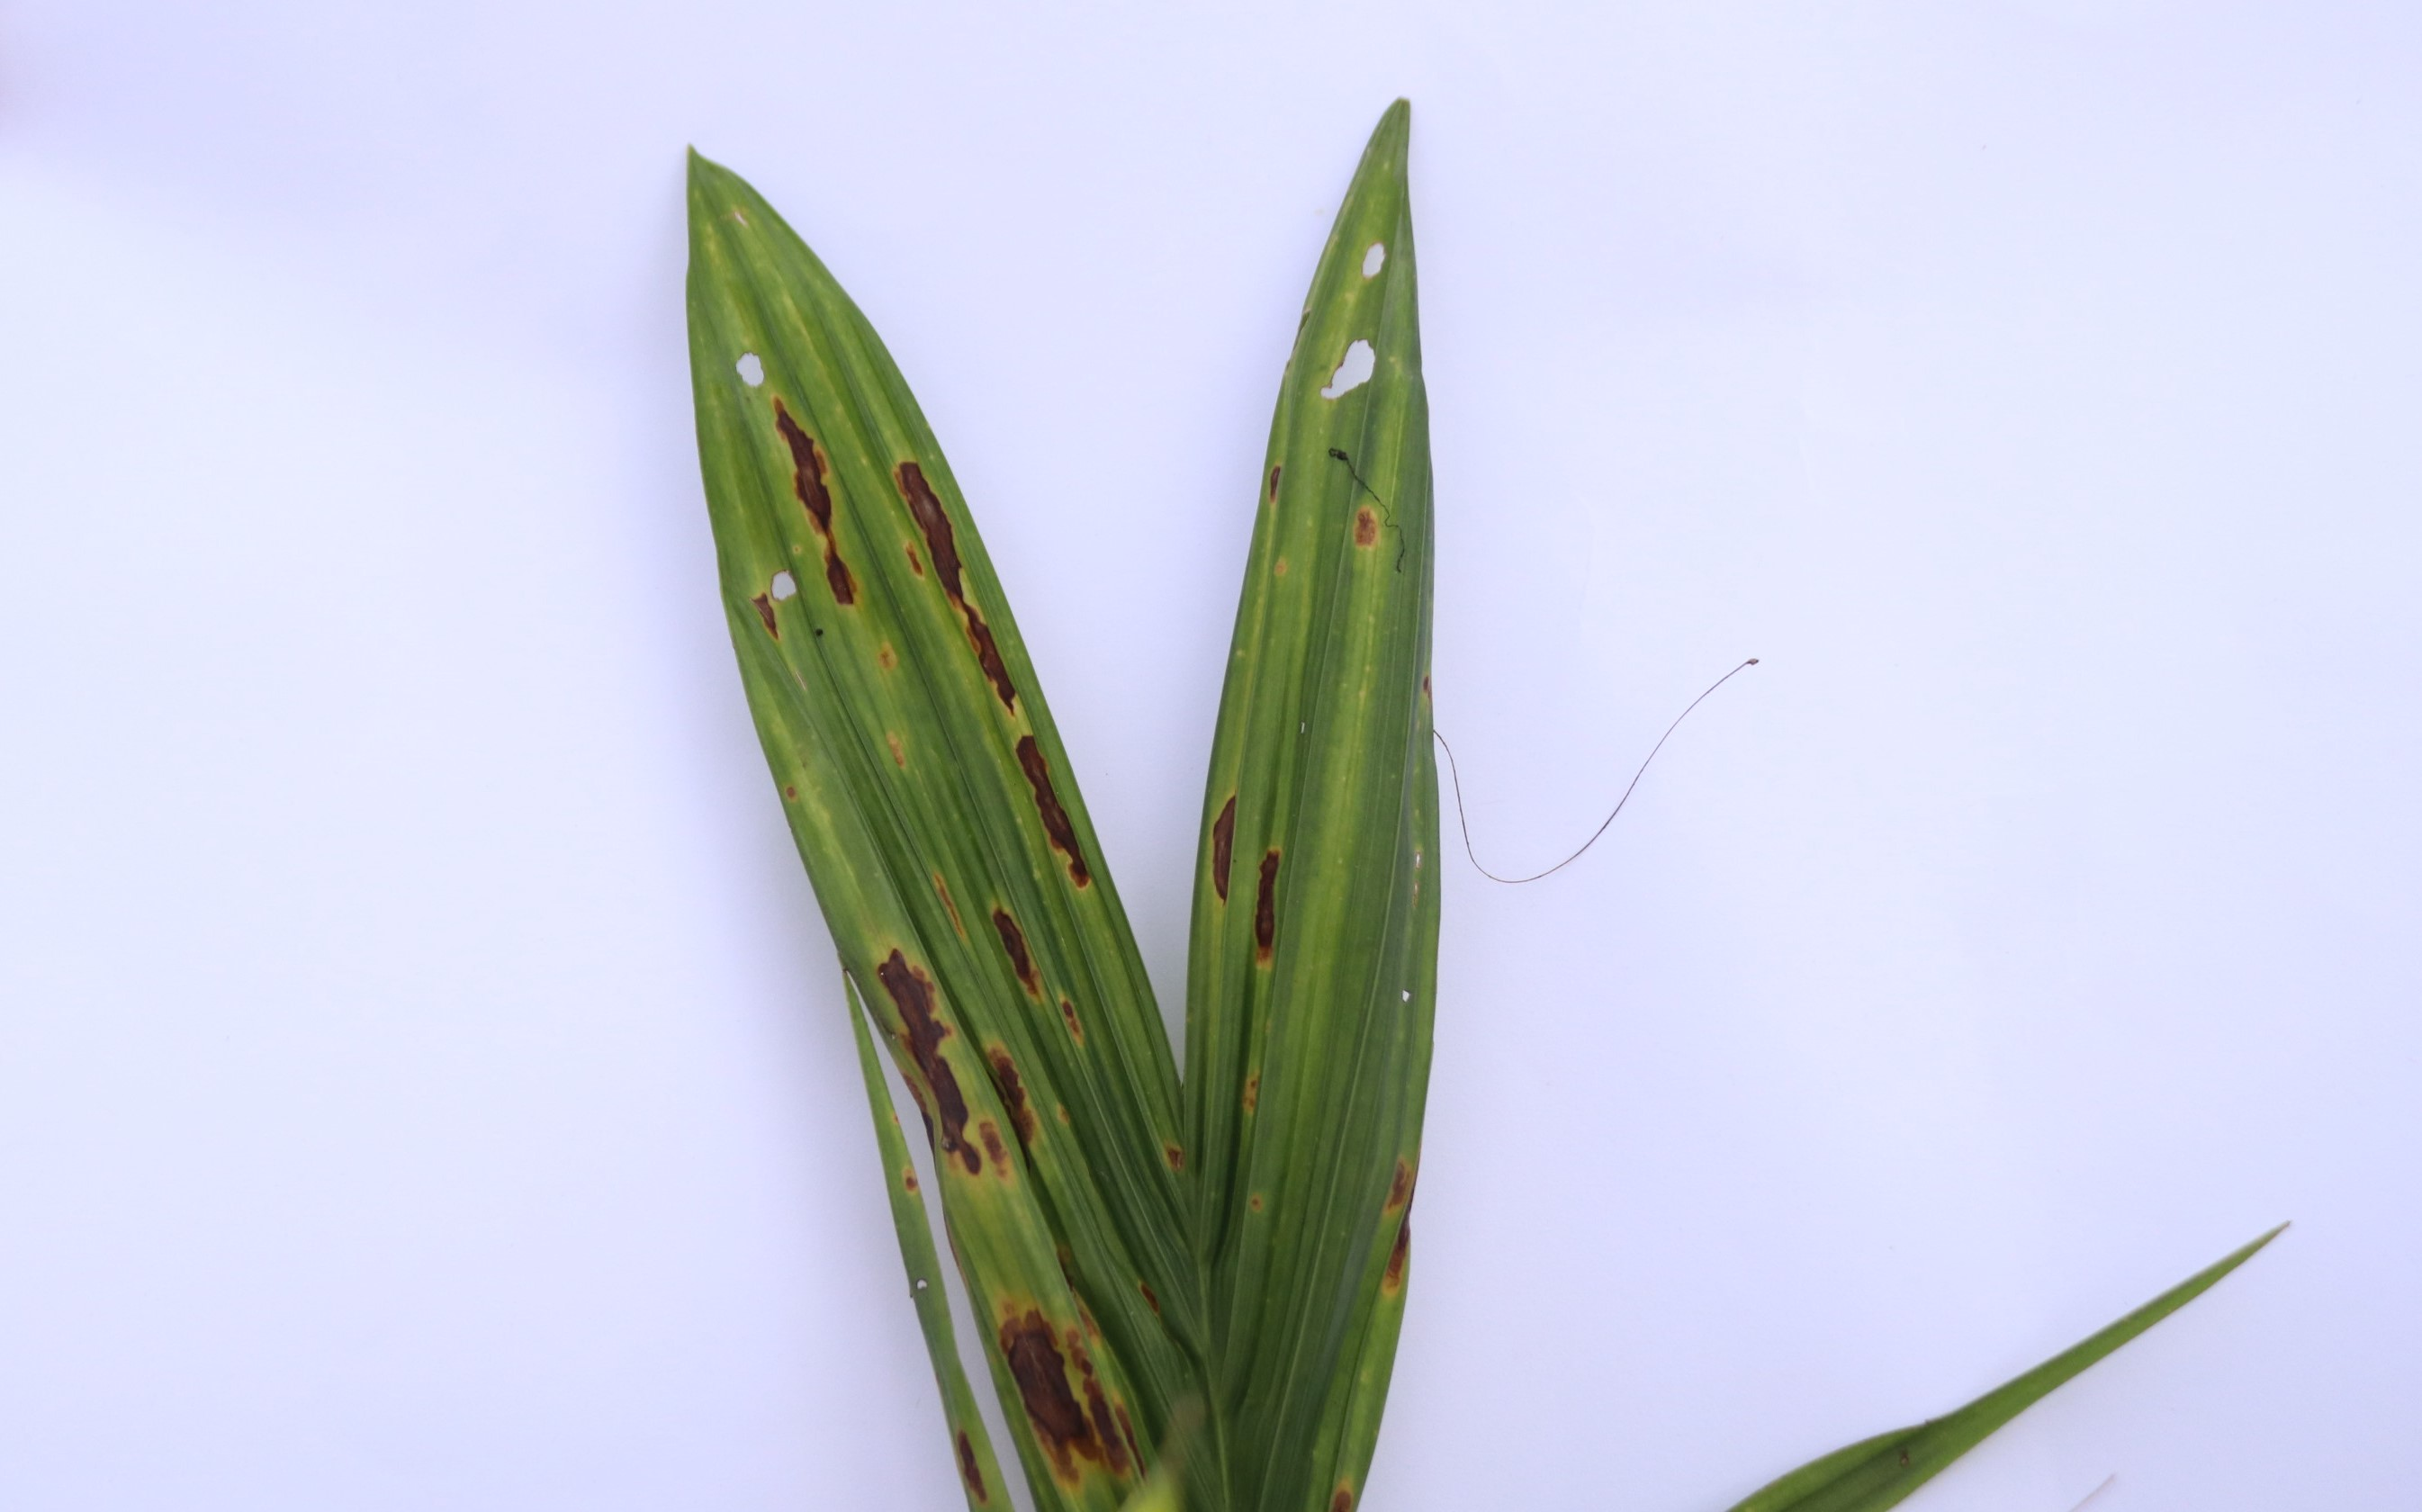
\includegraphics[width=0.22\textwidth]{figure/chapter-2-bercak-daun.jpg} & 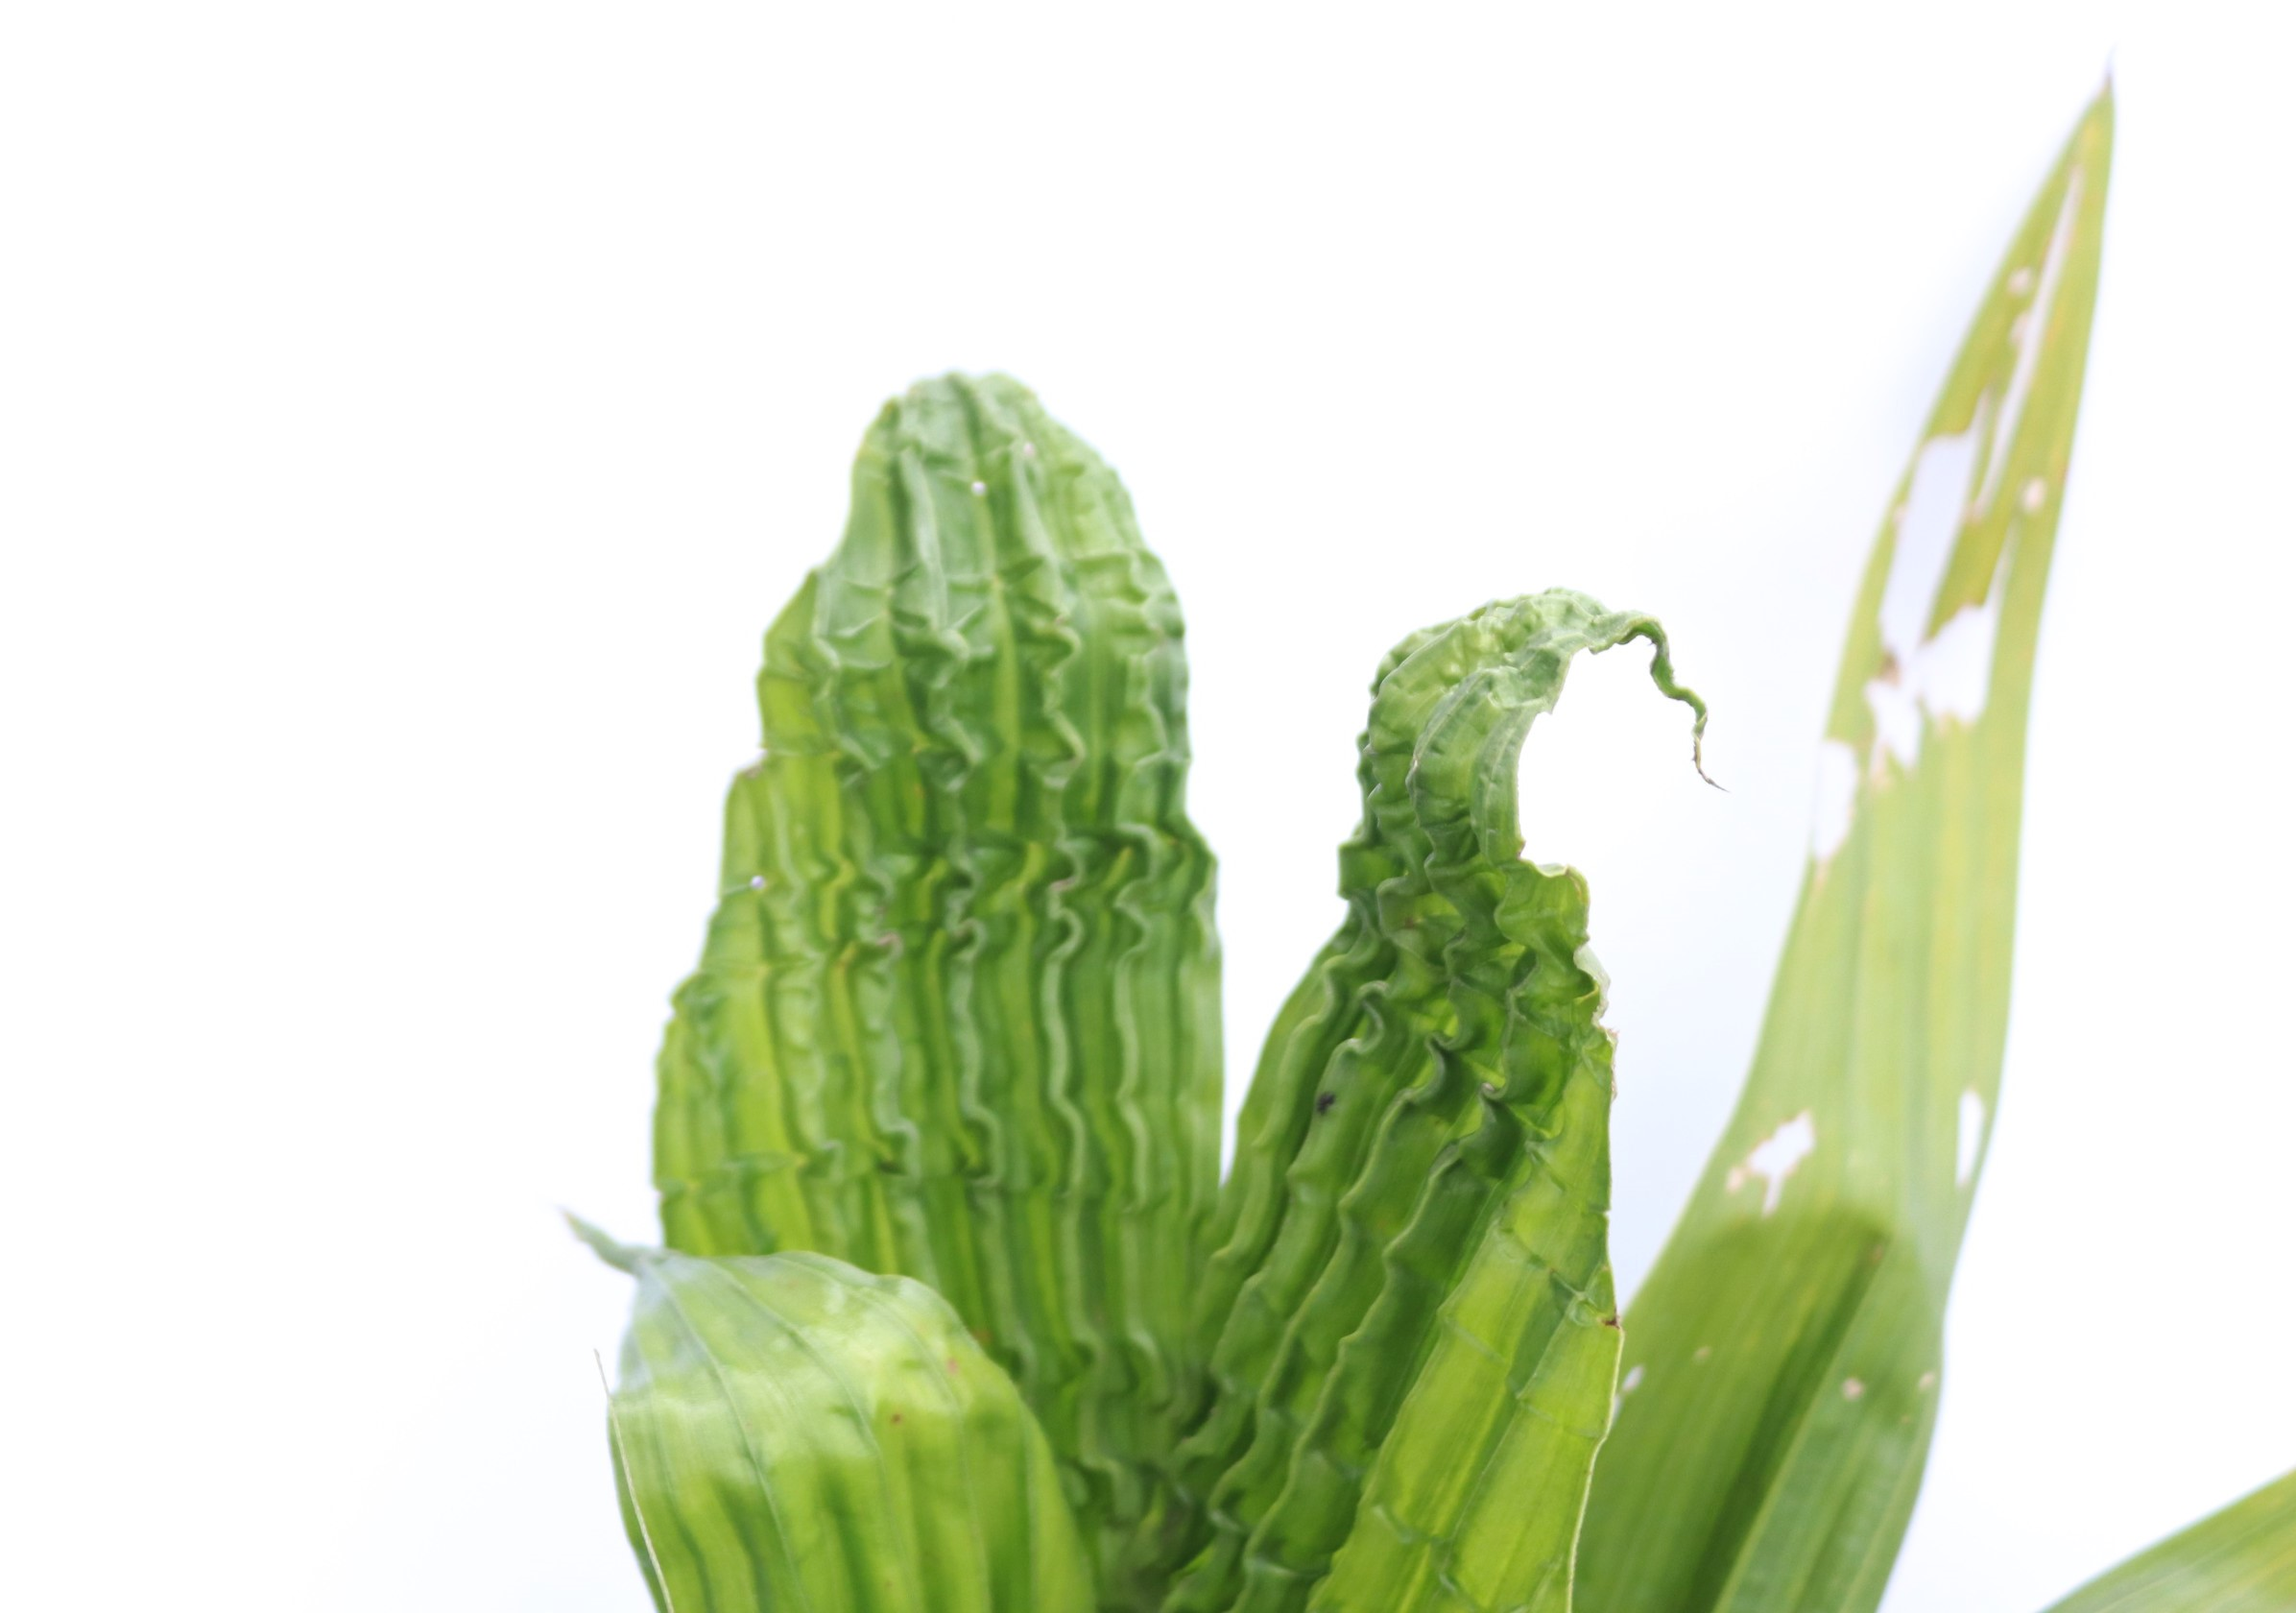
\includegraphics[width=0.22\textwidth]{figure/chapter-2-daun-berkerut.jpg} \\
		\small Bercak Daun & \small Daun Berkerut \\
		\hline
		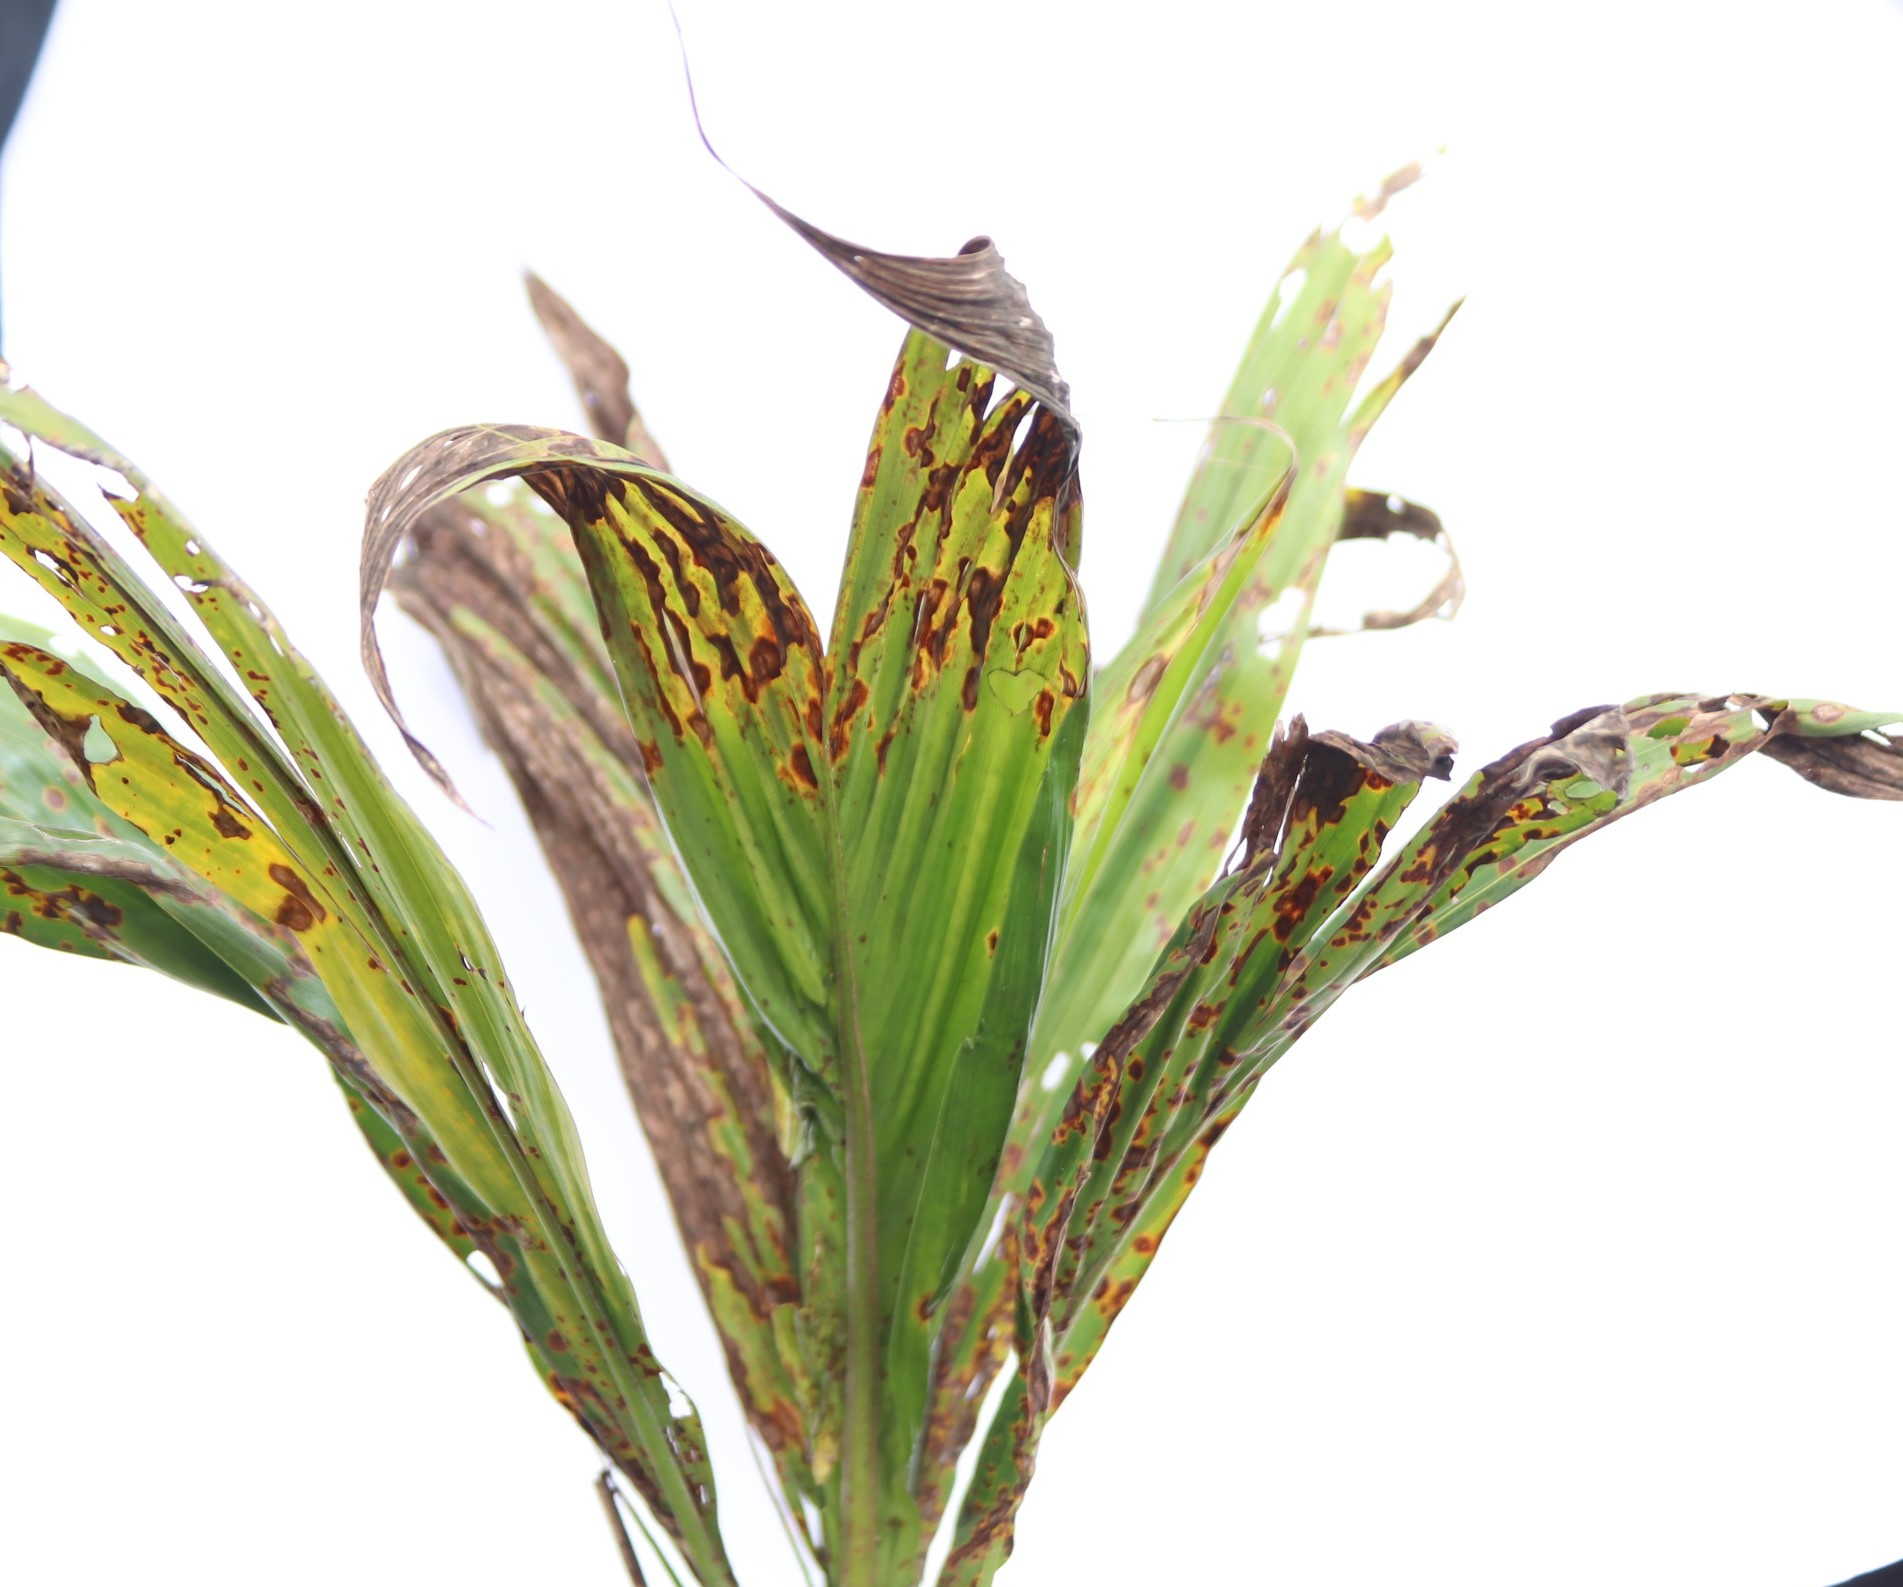
\includegraphics[width=0.22\textwidth]{figure/chapter-2-daun-berputar.jpg} & 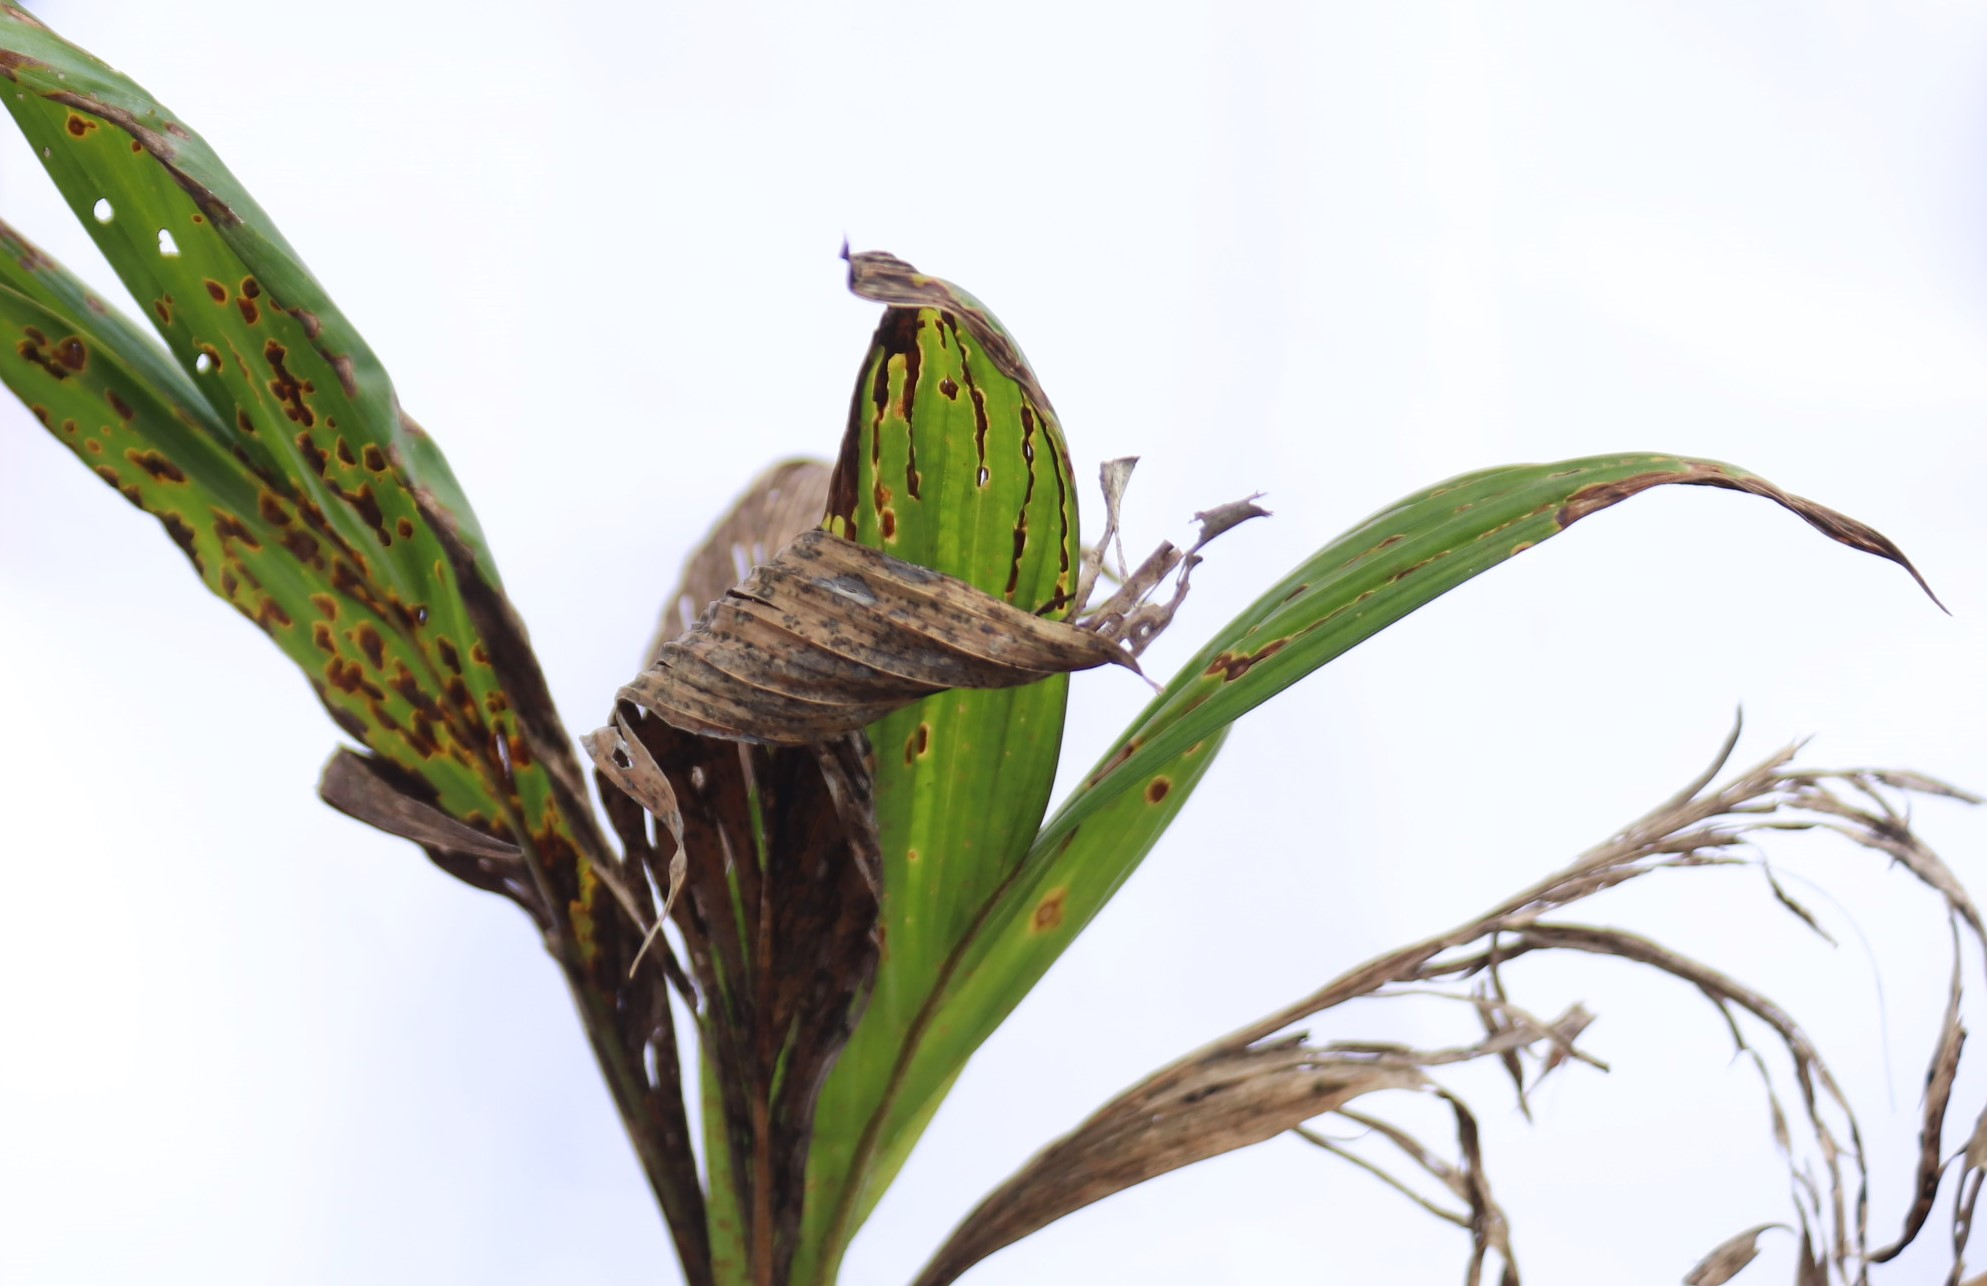
\includegraphics[width=0.22\textwidth]{figure/chapter-2-daun-menggulung.jpg} \\
		\small Daun Berputar & \small Daun Menggulung \\
		\hline
		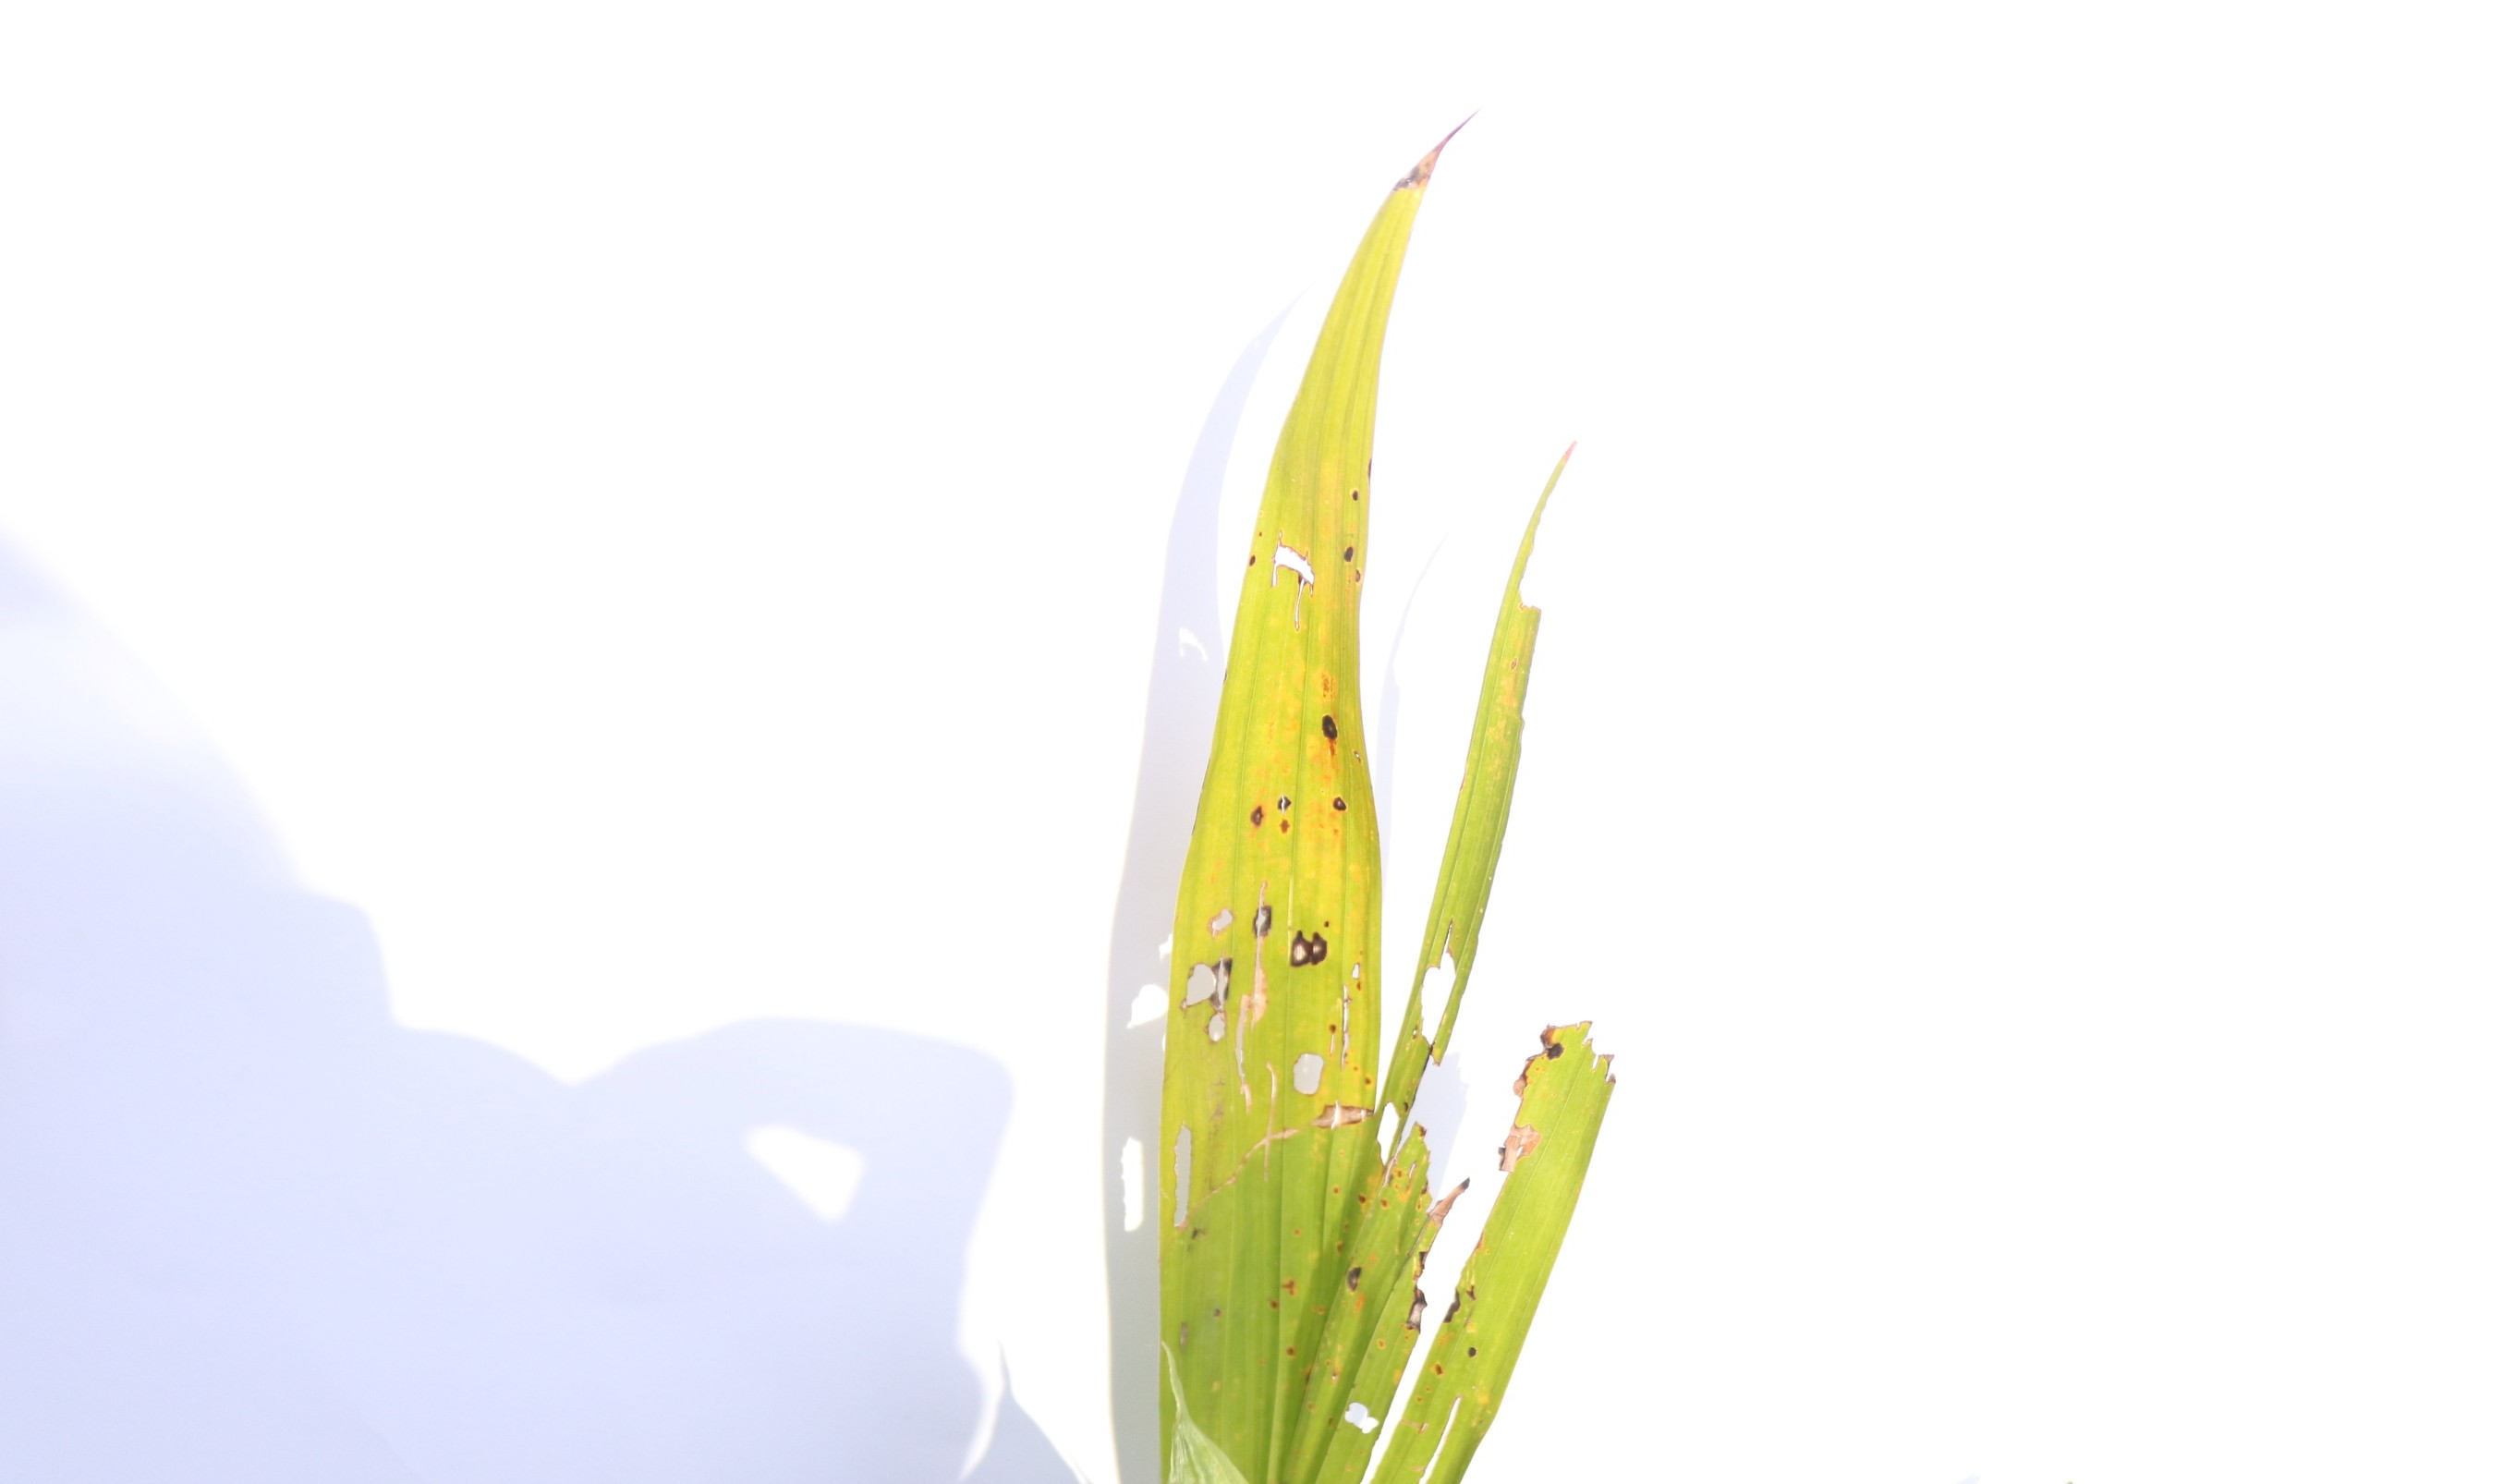
\includegraphics[width=0.22\textwidth]{figure/chapter-2-daun-menguning.jpg} & {} \\
		\small Daun Menguning & \\
		\hline
	\end{tabular}
	\caption{Foto Dataset Daun Bibit Kelapa Sawit}
	\label{tab:tabel-foto}
\end{table}

\section{Metode Tugas Akhir} \label{III.Metode}
Metode yang digunakan dalam penelitian ini terdiri dari beberapa tahapan utama, yaitu augmentasi data, segmentasi citra, ekstraksi fitur, identifikasi menggunakan \textit{Naïve Bayes Gaussian}, optimasi model dengan \textit{Genetic Algorithm} (GA) dan \textit{Particle Swarm Optimization} (PSO), serta evaluasi menggunakan \textit{confusion matrix}. Berikut penjelasan setiap tahapan:

\begin{enumerate}[noitemsep]
	\item  Augmentasi Data:  Proses augmentasi citra dilakukan menggunakan platform Roboflow untuk memperbanyak dan memperkaya variasi dataset. Teknik augmentasi yang digunakan meliputi rotasi, \textit{flipping, shear}, dan perubahan kecerahan, sehingga model dapat belajar dari data yang lebih beragam dan mengurangi risiko \textit{overfitting}.
	\item  Segmentasi Citra:  Segmentasi citra dilakukan secara otomatis menggunakan \textit{library Rembg} untuk menghapus latar belakang, kemudian dilakukan penyempurnaan secara manual melalui website Photoroom agar objek daun kelapa sawit terpisah sempurna dari latar belakang.
	\item  Ekstraksi Fitur:  Fitur warna dan tekstur diekstraksi dari citra hasil segmentasi. Fitur warna diambil dari rata-rata nilai RGB, sedangkan fitur tekstur diperoleh menggunakan metode \textit{Gray Level Co-occurrence Matrix (GLCM)}.
	\item  Klasifikasi \textit{Naïve Bayes Gaussian}:  Model klasifikasi utama yang digunakan adalah \textit{Naïve Bayes Gaussian}, yang menghitung probabilitas setiap kelas penyakit berdasarkan distribusi normal dari fitur yang diekstraksi.
	\item  Optimasi Model:  Untuk meningkatkan akurasi, parameter model \textit{Naïve Bayes} dioptimasi menggunakan dua algoritma metaheuristik, yaitu \textit{Genetic Algorithm} (GA) dan \textit{Particle Swarm Optimization} (PSO). Kedua metode ini digunakan untuk mencari parameter terbaik yang memaksimalkan performa klasifikasi.
	\item Evaluasi Model:  Evaluasi performa model dilakukan menggunakan \textit{confusion matrix} yang menghasilkan metrik akurasi, presisi, recall, dan F1-score untuk menilai efektivitas model dalam mengidentifikasi penyakit pada daun bibit kelapa sawit.
\end{enumerate}

Metode ini dirancang agar proses identifikasi penyakit pada daun bibit kelapa sawit dapat dilakukan secara otomatis, akurat, dan dapat diimplementasikan pada aplikasi berbasis web.

\section{Ilustrasi Perhitungan Metode} \label{III.Ilustrasi Perhitungan Metode}
Ilustrasi perhitungan metode yang digunakan dalam penelitian ini adalah sebagai berikut:

\subsection{Ekstraksi Fitur Warna} \label{III.Ekstraksi Fitur Warna}
Ekstraksi fitur warna pada penelitian ini dilakukan dengan menghitung rata-rata nilai RGB dari citra daun bibit kelapa sawit. Sebagai ilustrasi, proses ekstraksi nilai RGB dapat dijelaskan melalui contoh citra berukuran 4x4 piksel seperti yang ditunjukkan pada Tabel \ref{tab:tabel-rgb} berikut.
\begin{table}[H]
    \centering
    \begin{tabular}{|c|c|c|c|}
        \hline
        {[}155, 48, 201{]} & {[}92, 210, 35{]} & {[}18, 130, 245{]} & {[}233, 79, 12{]} \\
        {[}64, 188, 251{]} & {[}111, 22, 167{]} & {[}219, 143, 88{]} & {[}53, 199, 71{]} \\
        {[}176, 31, 238{]} & {[}85, 250, 96{]} & {[}40, 165, 15{]} & {[}205, 58, 124{]} \\
        {[}25, 140, 67{]} & {[}248, 103, 191{]} & {[}70, 14, 215{]} & {[}135, 228, 49{]} \\
        \hline
    \end{tabular}
    \caption{Tabel nilai RGB dalam format [R, G, B]}
    \label{tab:tabel-rgb}
\end{table}

\subsubsection{Nilai Rata-rata RGB} \label{III.Nilai Rata-rata RGB}
Selanjutnya, dilakukan perhitungan rata-rata untuk masing-masing komponen R, G, dan B dari seluruh piksel pada citra tersebut menggunakan metode averaging.

\begin{equation*}
\begin{split}
R &= \frac{155 + 92 + 18 + 233 + 64 + 111 + 219 + 53}{16} \\
  &+ \frac{176 + 85 + 40 + 205 + 25 + 248 + 70 + 135}{16} \\
  &= \frac{2134}{16} \\
  &= 133.375
\end{split}
\end{equation*}

\begin{equation*}
\begin{split}
G &= \frac{48 + 210 + 130 + 79 + 188 + 22 + 143 + 199}{16} \\
  &+ \frac{31 + 250 + 165 + 58 + 140 + 103 + 14 + 228}{16} \\
  &= \frac{2008}{16} \\
  &= 125.5
\end{split}
\end{equation*}

\begin{equation*}
\begin{split}
B &= \frac{201 + 35 + 245 + 12 + 251 + 167 + 88 + 71}{16} \\
  &+ \frac{238 + 96 + 15 + 124 + 67 + 191 + 215 + 49}{16} \\
  &= \frac{2065}{16} \\
  &= 129.0625
\end{split}
\end{equation*}

\subsubsection{Normalisasi Nilai Rata-rata RGB} \label{III.Normalisasi Nilai Rata-rata RGB}
Setelah diperoleh nilai rata-rata untuk setiap \textit{channel} warna (R, G, dan B), langkah selanjutnya adalah melakukan normalisasi terhadap nilai rata-rata tersebut. Normalisasi bertujuan agar nilai rata-rata RGB berada pada rentang yang seragam (misal 0–1), sehingga fitur warna yang dihasilkan menjadi lebih representatif dan tidak terpengaruh oleh skala intensitas piksel.

\begin{equation*}
\begin{aligned}
R &= \frac{133.375}{133.375 + 125.5 + 129.0625} \\
  &= \frac{133.375}{387.9375} \\
  &= 0.343
\end{aligned}
\end{equation*}

\begin{equation*}
\begin{aligned}
G &= \frac{125.5}{133.375 + 125.5 + 129.0625} \\
  &= \frac{125.5}{387.9375} \\
  &= 0.323
\end{aligned}
\end{equation*}

\begin{equation*}
\begin{aligned}
B &= \frac{129.0625}{133.375 + 125.5 + 129.0625} \\
  &= \frac{129.0625}{387.9375} \\
  &= 0.332
\end{aligned}
\end{equation*}


\subsection{Ekstraksi Fitur Tekstur} \label{III.Ekstraksi Fitur Tekstur}
Ekstraksi fitur tekstur dilakukan menggunakan metode \textit{Gray Level Co-occurrence Matrix} (GLCM). Setelah citra diubah ke \textit{grayscale}, GLCM dihitung untuk memperoleh fitur tekstur utama seperti kontras, korelasi, energi, dan homogenitas. Nilai-nilai ini kemudian digunakan sebagai input pada model klasifikasi. Contoh nilai RGB yang digunakan dapat dilihat pada Tabel \ref{tab:tabel-rgb} di bawah.
\begin{table}[h!]
\centering
\begin{tabular}{|c|c|c|c|}
\hline
[155, 48, 201] & [92, 210, 35] & [18, 130, 245] & [233, 79, 12] \\
\hline
[64, 188, 251] & [111, 22, 167] & [219, 143, 88] & [53, 199, 71] \\
\hline
[176, 31, 238] & [85, 250, 96] & [40, 165, 15] & [205, 58, 124] \\
\hline
[25, 140, 67] & [248, 103, 191] & [70, 14, 215] & [135, 228, 49] \\
\hline
\end{tabular}
\caption{Tabel nilai RGB dari citra 4x4}
\end{table}

\subsubsection{RGB menjadi Grayscale} \label{III.RGB menjadi Grayscale}
Untuk mengekstrak nilai tekstur, pertama kita akan mengubah citra tersebut dari RGB menjadi \textit{grayscale} dengan menggunakan rumus berikut:
\[
\text{Grayscale} = (0.2989 \times \text{Red}) + (0.5870 \times \text{Green}) + (0.1140 \times \text{Blue})
\]

Pemilihan rumus konversi RGB ke \textit{grayscale} ini didasarkan pada analisis kritis terhadap beberapa alternatif yang tersedia. \textit{Formula luminance} dari standar ITU-R BT.601 dipilih karena mempertimbangkan respons non-linear mata manusia terhadap berbagai panjang gelombang cahaya, yang sangat relevan untuk deteksi anomali warna pada daun. Dengan bobot yang proporsional terhadap sensitivitas retina manusia, yaitu 0.5870 untuk hijau, 0.2989 untuk merah, dan 0.1140 untuk biru. Formula ini memungkinkan pemisahan fitur patologis yang lebih presisi dibandingkan metode sederhana seperti rata-rata aritmatik RGB (R+G+B)/3 yang mengabaikan perbedaan persepsi warna.

Pendekatan ini secara signifikan meningkatkan kualitas ekstraksi fitur tekstur pada tahap selanjutnya, terutama untuk mengidentifikasi perbedaan subtil pada pola gejala penyakit daun kelapa sawit yang seringkali sulit dibedakan dengan metode konversi konvensional. Meskipun metode ini memerlukan komputasi lebih kompleks dibandingkan fungsi bawaan \textit{library} seperti OpenCV, pengorbanan efisiensi tersebut terbukti sepadan dengan peningkatan akurasi dalam konteks penelitian ini. Evaluasi komparatif yang dilakukan menunjukkan bahwa metode ini memberikan nilai kontras dan homogenitas GLCM yang lebih representatif pada citra daun dengan berbagai tingkat keparahan penyakit.

Berikut adalah contoh perhitungan yang dilakukan pada salah satu piksel dengan nilai RGB (155, 48, 201) dari citra yang didapatkan di atas, maka nilai \textit{grayscale} dihitung sebagai berikut:
\[
\text{Grayscale} = (0.2989 \times 155) + (0.5870 \times 48) + (0.1140 \times 201)
\]

Berikut adalah hasil konversi citra RGB menjadi grayscale, sebagaimana ditampilkan pada Tabel \ref{tab:tabel-grayscale} di bawah ini:
\begin{table}[H]
\centering
\begin{tabular}{|c|c|c|c|}
\hline
	97.42  & 154.76 & 109.62 & 117.39 \\ \hline
	158.11 & 65.14  & 159.41 & 140.75 \\ \hline
	97.94  & 183.10 & 110.52 & 109.46 \\ \hline
	97.29  & 156.36 & 53.65  & 179.77 \\ \hline
\end{tabular}
\caption{Tabel nilai grayscale dari citra RGB}
\label{tab:tabel-grayscale}
\end{table}

\subsubsection{Kuantisasi Nilai Pixel} \label{III.Kuantisasi Nilai Pixel}
Setelah matriks citra dikonversi ke \textit{grayscale}, langkah selanjutnya adalah melakukan kuantisasi nilai setiap piksel menggunakan metode kuantisasi uniform. Proses kuantisasi ini bertujuan untuk menyederhanakan rentang nilai piksel menjadi beberapa tingkat (level) tertentu agar perhitungan fitur tekstur pada tahap berikutnya menjadi lebih mudah dan efisien. Hasil kuantisasi nilai piksel \textit{grayscale} dapat dilihat pada Tabel \ref{tab:tabel-numerik} di bawah.

\begin{table}[H]
\centering
\begin{tabular}{|c|c|c|c|}
	\hline
	1 & 2 & 1 & 1 \\ \hline
	2 & 1 & 2 & 2 \\ \hline
	1 & 2 & 1 & 1 \\ \hline
	1 & 2 & 0 & 2 \\ \hline
\end{tabular}
\caption{Kuantisasi Nilai Pixel Grayscale}
\label{tab:tabel-numerik}
\end{table}

\subsubsection{Matriks \textit{Co-occurrence}} \label{III.Kuantisasi Nilai Pixel}
Selanjutnya, matriks (\textit{co-occurrence matrix}) dibangun untuk merepresentasikan hubungan spasial antara piksel referensi dan piksel tetangga dengan sudut 0 derajat serta jarak spasial 1. Hasil konstruksi matriks ini dapat dilihat pada Tabel~\ref{tab:MatriksCo-occurrence} di bawah.
\begin{table}[H]
\centering
\begin{tabular}{|c|c|c|c|c|}
\hline
\cellcolor{gray!20}i,j & \cellcolor{gray!20}0 & \cellcolor{gray!20}1 & \cellcolor{gray!20}2 & \cellcolor{gray!20}3 \\
\hline
\cellcolor{gray!20}0 & 0 & 0 & 1 & 0 \\
\hline
\cellcolor{gray!20}1 & 0 & 2 & 4 & 0 \\
\hline
\cellcolor{gray!20}2 & 1 & 3 & 1 & 0 \\
\hline
\cellcolor{gray!20}3 & 0 & 0 & 0 & 0 \\
\hline
\end{tabular}
\caption{Matriks \textit{Co-occurrence}}
\label{tab:MatriksCo-occurrence}
\end{table}


\subsubsection{Matriks Transpose dari Matriks \textit{Co-occurrence}} \label{III.Matriks Transpose dari Matriks Co-occurrence}
Selanjutnya, hasil dari matriks \textit{co-occurrence} di transpose, yang artinya hasil dari pertukaran baris dan kolom pada matriks \textit{co-occurrence}. Matriks ini digunakan untuk menghitung fitur tekstur yang lebih lanjut. Hasil matriks transpose dapat dilihat pada Tabel \ref{tab:MatriksTranspose} di bawah.

\begin{table}[H]
\centering
\begin{tabular}{|c|c|c|c|}
\hline
	0 & 0 & 1 & 0 \\ \hline
	0 & 2 & 3 & 0 \\ \hline
	1 & 4 & 1 & 0 \\ \hline
	0 & 0 & 0 & 0 \\ \hline
\end{tabular}
\caption{Matriks Transpose}
\label{tab:MatriksTranspose}
\end{table}

\subsubsection{Matriks Simetris} \label{III.Matriks Transpose dari Matriks Co-occurrence}
Selanjutnya, hasil matriks yang sebelumnya di transpose, kemudian dijumlahkan dengan matriks \textit{co-occurrence} yang telah dibangun sebelumnya. Hasil dari penjumlahan ini adalah matriks simetris yang digunakan untuk menghitung fitur tekstur lebih lanjut. Hasil dari matriks simetris dapat dilihat pada Tabel \ref{tab:MatriksSimetris} di bawah.

\begin{table}[H]
\centering
\begin{tabular}{|c|c|c|c|}
\hline
0 & 0 & 1 & 0 \\ \hline
0 & 2 & 3 & 0 \\ \hline
1 & 4 & 1 & 0 \\ \hline
0 & 0 & 0 & 0 \\ \hline
\end{tabular}
\caption{Matriks Simetris}
\label{tab:MatriksSimetris}
\end{table}

\subsubsection{Normalisasi Matriks Simetris} \label{III.Normalisasi Matriks Simetris}
Matriks simetris yang telah dibangun sebelumnya kemudian dinormalisasi dengan membagi setiap elemen pada matriks dengan jumlah total elemen pada matriks tersebut. Hasil dari normalisasi ini adalah matriks probabilitas yang digunakan untuk menghitung fitur tekstur lebih lanjut. Hasil dari normalisasi matriks simetris dapat dilihat pada Tabel \ref{tab:MatriksNormalisasi} di bawah.

\begin{figure}[H]
\centering
\textit{Total} $= 0 + 0 + 2 + 0 + 0 + 4 + 7 + 0 + 2 + 7 + 2 + 0 + 0 + 0 + 0 + 0$ \\
\textit{Total} $= 24$	
\end{figure}

\begin{table}[H]
\centering
\begin{tabular}{|c|c|c|c|}
\hline
$\frac{0}{24}$ & $\frac{0}{24}$ & $\frac{2}{24}$ & $\frac{0}{24}$ \\
\hline
$\frac{0}{24}$ & $\frac{4}{24}$ & $\frac{7}{24}$ & $\frac{0}{24}$ \\
\hline
$\frac{2}{24}$ & $\frac{7}{24}$ & $\frac{2}{24}$ & $\frac{0}{24}$ \\
\hline
$\frac{0}{24}$ & $\frac{0}{24}$ & $\frac{0}{24}$ & $\frac{0}{24}$ \\
\hline
\end{tabular}
\caption{Matriks Normalisasi}
\label{tab:MatriksNormalisasi}
\end{table}

Berikut adalah hasil dari normalisasi matriks simetris yang telah dibangun sebelumnya. Hasil dari matriks normalisasi dapat dilihat pada Tabel \ref{tab:MatriksNormalisasi} di bawah.
\begin{table}[H]
\centering
\begin{tabular}{|c|c|c|c|}
\hline
0 & 0     & 0.083 & 0     \\
\hline
0 & 0.166 & 0.291 & 0     \\
\hline
0.083 & 0.291 & 0.083 & 0 \\
\hline
0 & 0     & 0     & 0     \\
\hline
\end{tabular}
\caption{Tabel Hasil Normalisasi}
\label{tab:MatriksNormalisasi}
\end{table}

\subsubsection{Menghitung Nilai Contrast, Correlation, Energy, dan Homogenitas} \label{III.Menghitung Nilai Contrast, Correlation, Energy, dan Homogenitas}

\section*{1. Contrast}

\begin{align*}
	\textit{Contrast} = \sum_{i=0}^{G-1} \sum_{j=0}^{G-1} P_{i,j}(i-j)^2
\end{align*}

\begin{center}
\begin{align*}
\textit{Contrast} = 
&\ (0 \times (0 - 0)^2) + (0 \times (0 - 1)^2) + (0.083 \times (0 - 2)^2) \\
& + (0 \times (0 - 3)^2) + (0 \times (1 - 0)^2) + (0.166 \times (1 - 1)^2) \\
& + (0.291 \times (1 - 2)^2) + (0 \times (1 - 3)^2) \\
& + (0.083 \times (2 - 0)^2) + (0.291 \times (2 - 1)^2) \\
& + (0.083 \times (2 - 2)^2) + (0 \times (2 - 3)^2) \\
& + (0 \times (3 - 0)^2) + (0 \times (3 - 1)^2) \\
& + (0 \times (3 - 2)^2) + (0 \times (3 - 3)^2)
\end{align*}

\begin{align*}
\textit{Contrast} =
&\ 0 + 0 + 0.332 + 0 + 0 + 0 + 0.291 + 0 + 0.332 \\
& + 0.291 + 0 + 0 + 0 + 0 + 0 + 0
\end{align*}
\textit{Contrast} = 1.246
\end{center}

% -----
\section*{2. Correlation}

\[
\mu_i = \sum_{i=0}^{G-1} \sum_{j=0}^{G-1} i \cdot P_{i,j}
\]

\begin{align*}
\mu_i &= (0 \times 0) + (0 \times 0.083) + (0 \times 0) + (1 \times 0) \\
&\quad + (1 \times 0.166) + (1 \times 0.291) + (1 \times 0) \\
&\quad + (2 \times 0.083) + (2 \times 0.291) + (2 \times 0.083) \\
&\quad + (2 \times 0) + (3 \times 0) + (3 \times 0) \\
&\quad + (3 \times 0) + (3 \times 0) \\
&= 0 + 0 + 0 + 0 \\
&\quad + 0.166 + 0.291 + 0 \\
&\quad + 0.166 + 0.582 + 0.166 \\
&\quad + 0 + 0 + 0 + 0 + 0 \\
&= 1.371
\end{align*}

\[
\mu_j = \sum_{i=0}^{G-1} \sum_{j=0}^{G-1} j \cdot P_{i,j}
\]

\begin{align*}
\mu_j &= (0 \times 0) + (1 \times 0) + (2 \times 0.083) + (3 \times 0) \\
&\quad + (0 \times 0) + (1 \times 0.166) + (2 \times 0.291) + (3 \times 0) \\
&\quad + (0 \times 0.083) + (1 \times 0.291) + (2 \times 0.083) + (3 \times 0) \\
&\quad + (0 \times 0) + (1 \times 0) + (2 \times 0) + (3 \times 0) \\
&= 0 + 0 + 0.166 + 0 \\
&\quad + 0 + 0.166 + 0.582 + 0 \\
&\quad + 0 + 0.291 + 0.166 + 0 \\
&\quad + 0 + 0 + 0 + 0 \\
&= 1.371
\end{align*}


\[
\sigma_i^2 = \sum_{i=0}^{G-1} \sum_{j=0}^{G-1} (i - \mu_i)^2 \cdot P_{i,j}
\]

\begin{align*}
\sigma_i^2 &= ((0 - 1.371)^2 \times 0) + ((0 - 1.371)^2 \times 0) \\
&\quad + ((0 - 1.371)^2 \times 0.083) + ((0 - 1.371)^2 \times 0) \\
&\quad + ((1 - 1.371)^2 \times 0) + ((1 - 1.371)^2 \times 0.166) \\
&\quad + ((1 - 1.371)^2 \times 0.291) + ((1 - 1.371)^2 \times 0) \\
&\quad + ((2 - 1.371)^2 \times 0.083) + ((2 - 1.371)^2 \times 0.291) \\
&\quad + ((2 - 1.371)^2 \times 0.083) + ((2 - 1.371)^2 \times 0) \\
&= 0.156010003 + 0.022848406 + 0.040050831 + 0.032838003 \\
&\quad + 0.115141671 + 0.032838003 \\
&= 0.399726917
\end{align*}

\[
\sigma_j^2 = \sum_{i=0}^{G-1} \sum_{j=0}^{G-1} (j - \mu_j)^2 \cdot P_{i,j}
\]

\begin{align*}
\sigma_j^2 &= ((0 - 1.371)^2 \times 0) + ((1 - 1.371)^2 \times 0) \\
&\quad + ((2 - 1.371)^2 \times 0.083) + ((3 - 1.371)^2 \times 0) \\
&\quad + ((0 - 1.371)^2 \times 0) + ((1 - 1.371)^2 \times 0.166) \\
&\quad + ((2 - 1.371)^2 \times 0.291) + ((3 - 1.371)^2 \times 0) \\
&\quad + ((0 - 1.371)^2 \times 0.083) + ((1 - 1.371)^2 \times 0.291) \\
&\quad + ((2 - 1.371)^2 \times 0.083) + ((3 - 1.371)^2 \times 0) \\
&= 0.032838003 + 0.022848406 + 0.115141671 + 0.156010003 \\
&\quad + 0.040050831 + 0.032838003 \\
&= 0.399726917
\end{align*}

\[
\text{Correlation} = \sum_{i=0}^{G-1} \sum_{j=0}^{G-1} P_{i,j} \frac{(i - \mu_i)(j - \mu_j)}{\sqrt{(\sigma_i^2)(\sigma_j^2)}}
\]

\begin{align*}
\text{Correlation} &= 0 \times \frac{(0 - 1.371)(0 - 1.371)}{\sqrt{0.399 \cdot 0.399}} + 0 \times \frac{(0 - 1.371)(1 - 1.371)}{\sqrt{0.399 \cdot 0.399}} \\
&\quad + 0.083 \times \frac{(0 - 1.371)(2 - 1.371)}{\sqrt{0.399 \cdot 0.399}} + \ldots \\
&\quad + 0 \times \frac{(3 - 1.371)(3 - 1.371)}{\sqrt{0.399 \cdot 0.399}} \\
&= -0.559
\end{align*}

% -----
\section*{3. Energy}

\[
Energy = \sum_{i=0}^{G-1} \sum_{j=0}^{G-1} (P_{i,j})^2
\]

\begin{align*}
Energy &= (0)^2 + (0)^2 + (0.083)^2 + (0)^2 \\
&\quad + (0)^2 + (0.166)^2 + (0.291)^2 \\
&\quad + (0)^2 + (0)^2 + (0.083)^2 \\
&\quad + (0.291)^2 + (0.083)^2 \\
&\quad + (0)^2 + (0)^2 + (0)^2 + (0)^2 \\
&= 0.006889 + 0.027556 + 0.084681 + 0.006889 \\
&\quad + 0.084681 + 0.006889 \\
&= 0.217185
\end{align*}


% -----
\section*{4. Homogenity}

\[
Homogenity = \sum_{i=0}^{G-1} \sum_{j=0}^{G-1} \frac{P_{i,j}}{1 + (i - j)^2}
\]

\begin{align*}
Homogenity &= 
\frac{0}{1 + (0 - 0)^2} + \frac{0}{1 + (0 - 1)^2} \\
&\quad + \frac{0.083}{1 + (0 - 2)^2} + \frac{0}{1 + (0 - 3)^2} \\
&\quad + \frac{0}{1 + (1 - 0)^2} + \frac{0.166}{1 + (1 - 1)^2} \\
&\quad + \frac{0}{1 + (1 - 2)^2} + \frac{0}{1 + (1 - 3)^2} \\
&\quad + \frac{0.291}{1 + (2 - 1)^2} + \frac{0.083}{1 + (2 - 2)^2} \\
&\quad + \frac{0}{1 + (2 - 3)^2} + \frac{0}{1 + (2 - 0)^2} \\
&\quad + \frac{0.291}{1 + (3 - 2)^2} + \frac{0}{1 + (3 - 0)^2} \\
&\quad + \frac{0}{1 + (3 - 1)^2} + \frac{0}{1 + (3 - 3)^2} \\
\\
Homogenity &= 0.0166 + 0.166 + 0.1455 + 0.0166 \\
&\quad + 0.1455 + 0.083 \\
\\
Homogenity &= 0.5732
\end{align*}



